\documentclass[a4paper,10pt]{article}

\usepackage{tabularx}
\usepackage{graphicx}
\usepackage{geometry}
\geometry{
    top=2cm,
    bottom=2cm,
    left=1cm,
    right=1cm
}

\usepackage{xepersian}
\settextfont{Vazirmatn-Regular.ttf}

\title{ML4RE - یادگیری ماشین برای مهندسی نیازمندی‌ها}
\author{}
\date{}

\linespread{1.5}

\begin{document}

    \maketitle

    % MARK: abstract

    \begin{abstract}
        
        مقدمه: تحقیقات در زمینه یادگیری ماشین برای مهندسی نیازمندی‌ها (ML4RE) به تدریج توجه بیشتری از سوی محققان و عملی‌کنندگان به خود جلب کرده است. اگرچه تحقیقات پیشگامانه پتانسیل استفاده از تکنیک‌های یادگیری ماشین برای بهبود فرآیندهای مهندسی نیازمندی‌ها را نشان داده‌اند، اما یک مرور نظام‌مند و جامع از ادبیات علمی که دیدگاه صنعتی را نیز در بر گیرد، در دانشگاه‌ها وجود ندارد. به‌ویژه، هیچ‌یک از مرورهای موجود در زمینه ML4RE به ادبیات خاکستری که عمدتاً از منابع عملی‌کنندگان منشأ می‌گیرد و بازتاب‌دهنده مسائل و چالش‌های واقعی در عمل است، توجه نکرده‌اند.

        هدف: در این مقاله، ما یک بررسی نظام‌مند از انتشارات علمی در زمینه ML4RE انجام می‌دهیم و آن را با نظرات عملی‌کنندگان از Stack Overflow تکمیل می‌کنیم تا یک مرور جامع از ادبیات ارائه دهیم. هدف تحقیق ما ارائه یک دیدگاه جامع از پیشرفت‌های کنونی در تحقیقات ML4RE، بیان سوالات و چالش‌های اصلی در عمل مهندسی نیازمندی‌ها، درک فاصله بین تحقیق و عمل، و ارائه بینش‌های خود درباره چگونگی توسعه عملی این حوزه دانشگاهی در آینده است.

        روش: ما به صورت نظام‌مند 207 مقاله علمی در زمینه ML4RE از سال 2010 تا 2022 را بررسی کردیم و همچنین 375 سوال مرتبط با مهندسی نیازمندی‌ها در Stack Overflow و پاسخ‌های مربوطه را تحلیل کردیم. تحلیل ما شامل روندها، فعالیت‌ها و وظایف متمرکز بر مهندسی نیازمندی‌ها، راه‌حل‌های به‌کاررفته و داده‌های مرتبط بود. در نهایت، یک تحلیل مشترک انجام دادیم و نتایج هر دو بخش را با هم مقایسه کردیم.
        
        نتایج: بر اساس نتایج آماری از ادبیات جمع‌آوری‌شده، ما یک نقشه راه علمی را خلاصه کرده و تفاوت‌ها را تحلیل کردیم و توصیه‌های پژوهشی ارائه دادیم. پیشنهادات ما شامل توسعه دستیاران هوشمند پاسخگویی به سوالات با استفاده از مدل‌های زبان بزرگ، ادغام یادگیری ماشین در ابزارهای صنعتی و ترویج همکاری بین دانشگاه و صنعت است.

        نتیجه‌گیری: این مطالعه با ارائه یک دیدگاه جامع از ML4RE، بیان تفاوت‌های بین تحقیق و عمل، و پیشنهاد راه‌حل‌های عملی برای پر کردن شکاف بین دانشگاه و صنعت، به پیشرفت این حوزه کمک می‌کند.

    \end{abstract}

    % MARK: Introduction
    
    \section{مقدمه}

    مهندسی نیازمندی‌ها (RE) یک مرحله اساسی در مراحل اولیه مهندسی نرم‌افزار (SE) است. اگرچه پژوهشگران به طور مستمر در حال بررسی روش‌ها و تکنیک‌هایی برای تسهیل فرآیندهای نیازمندی هستند، اما کل فرآیند مهندسی نیازمندی‌ها همچنان نیاز به تلاش دستی زیادی دارد (مثلاً استخراج نیازمندی‌های ذی‌نفعان از طریق مصاحبه یا طبقه‌بندی نیازمندی‌ها بر اساس یک طبقه‌بندی خاص). دلیل اصلی این موضوع این است که فعالیت‌های RE معمولاً نیاز به دانش عمیق حوزه و مهارت‌های تحلیل پیشرفته دارند که به طور کامل قابل اتوماسیون نیست.

    در سال‌های اخیر، توسعه سریع فناوری یادگیری ماشین (ML) با بهبود قدرت محاسباتی تحریک شده است. کاربردهای موفق ML در زمینه‌هایی مانند پردازش زبان طبیعی، شناسایی تصویر و داده‌کاوی فرصت‌هایی را برای استفاده از تکنیک‌های ML در زمینه RE فراهم کرده است. استفاده از فناوری ML در RE یک رویکرد هوشمندانه‌تر و کارآمدتر برای مدیریت داده‌های نیازمندی‌ها ارائه می‌دهد. به عنوان مثال، ML می‌تواند در طبقه‌بندی خودکار نیازمندی‌ها کمک کند زیرا می‌تواند اطلاعات بالقوه نیازمندی‌ها را خلاصه کند.

    علاوه بر این، با توسعه سریع تکنیک‌های اطلاعاتی، کار و زندگی روزمره ما دیجیتالی می‌شوند. در نتیجه، داده‌های مرتبط با نیازمندی‌ها بیشتر و بیشتر دیجیتالی و به‌طور عمومی در دسترس قرار می‌گیرند، که پژوهش در زمینه یادگیری ماشین برای مهندسی نیازمندی‌ها (ML4RE) را ترویج می‌کند. به عنوان مثال، بررسی‌های کاربران از برنامه‌های موبایلی به طور گسترده‌ای برای استخراج نیازمندی‌های کاربران مورد بررسی قرار گرفته‌اند.

    تحقیقات قبلی ML4RE را مورد بررسی قرار داده‌اند. اقبال و همکاران [2] یک بررسی برای به‌دست‌آوردن نمای کلی از چگونگی کمک تکنیک‌های ML به فعالیت‌های RE انجام دادند. علاوه بر این، زمانی و همکاران [3] یک مطالعه نگاشت از کاربردهای ML در RE انجام دادند و 65 مقاله را برای ارزیابی اثربخشی ML در اتوماسیون وظایف RE تحلیل کردند. کارهای آن‌ها بر کل فرآیند RE متمرکز بود و نحوه تأثیرگذاری و تسهیل تکنیک‌های ML در مراحل مختلف را روشن کردند.

    به علاوه، برخی تحقیقات به فعالیت‌ها یا وظایف خاص RE می‌پردازند. به عنوان مثال، لیم و همکاران [4] رویکردهای پیشرفته فعلی برای استخراج نیازمندی‌های مبتنی بر داده از منابع داده پویا را بررسی کردند. ما متوجه شدیم که این مطالعات عمدتاً بر انتشارات علمی متمرکز بوده و از ادغام بینش‌های حاصل از منابع ادبیات خاکستری، مانند وبلاگ‌ها و انجمن‌های صنعتی غافل بوده‌اند.

    بر خلاف انتشارات علمی که عمدتاً توسط پژوهشگران منتشر می‌شوند، ادبیات خاکستری به‌طور مداوم توسط عملی‌کنندگان تولید می‌شود و بر "وضعیت عمل" نور می‌تاباند [5]. همان‌طور که در [6] اشاره شده، ادغام ادبیات خاکستری در مرورهای نظام‌مند ادبیات می‌تواند فاصله بین پژوهش‌های علمی و عملی را پر کند و دیدگاه جامع‌تری از چالش‌ها و راه‌حل‌ها ارائه دهد.

    اگرچه تعداد مرورهای نظام‌مند ادبیات که ادبیات خاکستری را در مطالعات SE در نظر گرفته‌اند در حال افزایش است [7,8]، اما در RE به اندازه کافی رایج نیستند. برای پر کردن این شکاف در زمینه RE، این مقاله قصد دارد یک مرور نظام‌مند از ادبیات در زمینه ML4RE انجام دهد که با بینش‌های حاصل از ادبیات خاکستری منابع شده از Stack Overflow تکمیل شود.

    هدف این مرور ادبیات سه بخشی است. بخش سفید شامل مرور 207 مقاله منتشر شده بین سال‌های 2010 تا 2022 است که به‌طور خاص بر ML4RE متمرکز است. در همین حال، بخش خاکستری شامل تحلیل 375 سوال و پاسخ‌های مربوطه جمع‌آوری شده از مباحث Stack Overflow درباره فعالیت‌های RE در همان دوره است. در نهایت، تحلیل مشترک ما شامل مقایسه نتایج این دو بخش برای تشخیص شباهت‌ها و تفاوت‌های آن‌ها است. ما روندها، فعالیت‌های RE، وظایف RE، راه‌حل‌ها و داده‌های موجود در ادبیات را تحلیل می‌کنیم.

    نتایج تحقیق نشان می‌دهد که هر دو بخش به تحلیل RE و مستندسازی نیازمندی‌ها علاقه‌مند هستند. فراتر از شباهت‌ها، بخش سفید تمایل به تمرکز بر استخراج نیازمندی‌ها دارد، در حالی که بخش خاکستری بیشتر بر مدیریت نیازمندی‌ها تأکید دارد. بخش سفید استفاده از تکنولوژی‌های ML مانند SVM، CNN و BERT را برجسته می‌کند. در مقابل، بخش خاکستری بیشتر بر ابزارهایی مانند Microsoft TFS، Jira و IBM Rational DOORS و تکنیک‌های ML مانند LDA، POS، TF-IDF و شبکه‌های عصبی تکیه دارد. علاوه بر این، بخش خاکستری توجه ویژه‌ای به داستان کاربر و مورد استفاده دارد که در بخش سفید نسبتاً کمتر مورد بررسی قرار گرفته است.

    بر اساس این یافته‌ها، ما یک نقشه راه علمی خلاصه کرده و تحلیل دقیقی از تفاوت‌های بین بخش سفید و خاکستری ارائه می‌دهیم. سپس پیشنهادات پژوهشی ارائه می‌دهیم، از جمله توسعه دستیاران هوشمند پاسخگویی به سوالات با استفاده از مدل‌های زبان بزرگ و ادغام یادگیری ماشین در ابزارهای صنعتی. همچنین، همکاری بیشتر بین دانشگاه و صنعت را برای درک عمیق‌تر مشکلات پژوهشی واقعی و داده‌ها تشویق می‌کنیم.

    در خلاصه، این مقاله چهار کمک اصلی را ارائه می‌دهد. اولاً، یک نمای جامع از وضعیت فعلی پژوهش‌های ML4RE ارائه می‌دهیم. دوماً، شرایط واقعی عملی‌کنندگان RE را از طریق ادبیات خاکستری حاصل از Stack Overflow بررسی می‌کنیم. سوماً، فاصله بین پژوهش و عمل در حوزه ML4RE را به‌ویژه در زمینه‌هایی که کمتر مورد توجه پژوهشگران قرار گرفته‌اند، برجسته می‌کنیم. و در نهایت، برای پر کردن فاصله بین صنعت و دانشگاه، پیشنهادات پژوهشی عملی در ML4RE ارائه می‌دهیم.

    در بخش‌های باقی‌مانده این مقاله، کارهای مرتبط را در بخش 2 ارائه می‌دهیم. بخش 3 پروتکل تحقیق برای مرور نظام‌مند ادبیات ما را ارائه می‌دهد. در سه بخش بعدی، نتایج این بررسی و پاسخ به سوالات پژوهشی را ارائه می‌دهیم. بخش 4 نتایج بخش سفید، بخش 5 بر بخش خاکستری تمرکز می‌کند و بخش 6 نتایج تحلیل مشترک را ارائه می‌دهد. بر اساس نتایج، در بخش 7 به بحث پرداخته و چندین پیشنهاد ارائه می‌دهیم. بخش 8 شامل تحلیل تهدیدات به اعتبار این بررسی است. در نهایت، مقاله را در بخش 9 نتیجه‌گیری می‌کنیم.
    
    % MARK: Related work

    \section{کارهای مرتبط}

    کارهای مرتبط با بررسی ادبیات ما در حوزه یادگیری ماشین برای مهندسی نیازمندی‌ها (ML4RE) از دو منبع مختلف به دست آمده است. مجموعه اول شامل بررسی‌های ادبیات مرتبط با ML4RE می‌باشد. مجموعه دوم شامل بررسی‌های سیستماتیکی ادبیات در حوزه مهندسی نرم‌افزار (SE) است. در دو زیربخش پیش رو، جزئیات کارهای مرتبط از این دو منبع را به طور دقیق ارائه خواهیم داد.

        \subsection{بررسی‌های ادبیات در مورد یادگیری ماشین برای مهندسی نیازمندی‌ها (ML4RE):}

            در این بخش، یک مجموعه از بررسی‌های ادبیات مرتبط با یادگیری ماشین برای مهندسی نیازمندی‌ها (ML4RE) را ارائه می‌دهیم. ما چندین بررسی ادبیات را پیدا کرده‌ایم، برخی به کلیه فرآیند مهندسی نیازمندی‌ها می‌پردازند، در حالی که برخی دیگر بر روی فعالیت‌ها یا وظایف خاص مهندسی نیازمندی‌ها تمرکز دارند. بنابراین، این زیربخش به دو بخش تقسیم شده است تا این کارها را به تفصیل معرفی کند.

            \subsubsection{فرآیند کامل مهندسی نیازمندی‌ها}

                دو مقاله به کلیه فرآیند مهندسی نیازمندی‌ها متمرکز شده‌اند و یک بررسی کلی از نحوه کاربرد تکنیک‌های یادگیری ماشین در مراحل مختلف مهندسی نیازمندی‌ها ارائه داده‌اند. در مقاله Iqbal و همکاران [2]، بررسی‌ای بر روی مقالات تحقیقاتی انجام شده است تا چگونگی کمک یادگیری ماشین به مهندسی نیازمندی‌ها را بررسی کند. آن‌ها تأثیر یادگیری ماشین را در پنج مرحله اصلی مهندسی نیازمندی‌ها مشاهده کرده و مسائل خاصی که توسط یادگیری ماشین حل شده‌اند، ویژگی‌ها، الگوریتم‌های ML و مجموعه داده‌ها را بررسی کرده‌اند. با این حال، مقالاتی که آن‌ها بررسی کردند از یک فرآیند جستجوی سیستماتیک به دست نیامده بودند و بنابراین، نتیجه‌گیری‌های به دست آمده ممکن است سیستماتیک و جامع نباشد.

                Zamani و همکاران [3] یک مطالعه نگاشتی از کاربردهای یادگیری ماشین در مهندسی نیازمندی‌ها انجام دادند، با تجزیه و تحلیل 65 مقاله برای ارزیابی کارآیی یادگیری ماشین در اتوماسیون وظایف مهندسی نیازمندی. این مطالعه تکنیک‌ها، چالش‌ها، مجموعه داده‌ها و معیارهای ارزیابی این مطالعات را شناسایی می‌کند. مقایسه با بررسی جامع ما، این مقاله بیشتر بر جنبه‌های تجربی یادگیری ماشین در مهندسی نیازمندی‌ها تمرکز دارد و بینش‌های خاصی را در کارآمدی عملی ML در این زمینه ارائه می‌دهد. علاوه بر این، مقاله Zhao و همکاران [9] بر روی NLP4RE تمرکز داشتند، با تحلیل 404 مطالعه برای درک کاربرد پردازش زبان طبیعی در مهندسی نیازمندی‌ها. با توجه به تداخلات بین NLP و ML، این تحقیق را به عنوان یکی از کارهای مرتبط برای تحلیل می‌پذیریم.
            
            
            \subsubsection{بخشی از فرآیند مهندسی نیازمندی‌ها}

                در فرآیند استخراج نیازمندی‌ها، G.C. Sampada و همکاران [10] یک نگاه کلی از رویکردهای مختلف برای اتوماسیون استخراج و مشخصه‌گذاری نیازمندی‌ها در چرخه توسعه نرم‌افزار ارائه دادند. Lim و همکاران [4] وضعیت فعلی روش‌های پیشروی استخراج نیازمندی‌های مبتنی بر داده از منابع داده پویا را بررسی کردند و شکاف‌های تحقیق را شناسایی کردند. Cheligeer و همکاران [11] با انتخاب 86 مقاله، مطالعاتی را که فناوری‌های ML و NLP را در استخراج نیازمندی‌ها شامل می‌شوند، خلاصه و تحلیل کردند. آن‌ها تکنیک‌های مختلف برای ساخت روش‌های استخراج نیازمندی مبتنی بر ML را به پنج بخش دسته‌بندی کردند.

                در فرآیند طبقه‌بندی نیازمندی‌ها، Alrumaih و همکاران [12] به بررسی مطالعات تحقیقی در زمینه طبقه‌بندی نیازمندی‌ها پرداختند و محدودیت‌ها را بررسی کردند تا پیشنهادهای بهبودی ارائه دهند. Perez و همکاران [13] کاربردهای تکنیک‌های ML در طبقه‌بندی نیازمندی‌های نرم‌افزار را بر اساس 13 مقاله بررسی کردند و الگوریتم‌های طبقه‌بندی مکررترین و مجموعه داده‌های آموزشی مکررترین را خلاصه کردند. Khelifa و همکاران [14] بررسی کردند که آیا تکنیک‌های یادگیری ماشین در طبقه‌بندی نیازمندی‌ها نرم‌افزاری و طبقه‌بندی درخواست‌های تغییرات نیازمندی‌ها قابل اعمال هستند. به علاوه، Kadebu و همکاران [15] بر روی مهندسی نیازمندی‌های امنیتی تمرکز کردند و کاربردهای تکنیک‌های ML در استخراج و طبقه‌بندی نیازمندی‌های امنیتی را بررسی کردند.

                در فرآیند مدیریت نیازمندی‌ها، Xu و همکاران [16] هشت روش ML را که در مدیریت نیازمندی‌ها استفاده شده است خلاصه کردند و 18 شاخص ارزیابی برای مدیریت نیازمندی‌ها در روش ML مشخص کردند. کار آن‌ها به عنوان یک درک اولیه از گستره‌ی وسیعی از تکنیک‌های ML در مدیریت نیازمندی‌ها خدمت می‌کند، در حالی که برخی مطالعات به تفصیل به وظایف خاص می‌پردازند.

                Achimugu و همکاران [17] به بررسی تکنیک‌های اولویت‌بندی نیازمندی‌های نرم‌افزار از طریق 73 مقاله مرتبط پرداختند و چندین محدودیت در تکنیک‌های اولویت‌بندی موجود را مورد بررسی قرار دادند. به علاوه، Li و همکاران [18] با انجام یک مطالعه نگاشت سیستماتیک با 26 مطالعه، 32 فناوری ML برای پیگیری نیازمندی‌ها را خلاصه کردند. از مطالب فوق مشخص است که تعداد زیادی از بررسی‌های ادبیات عالی در زمینه ML4RE وجود دارد. با این حال، در حال حاضر، کمبودی در تحقیقات وجود دارد که ادغام بخش خاکستری را که نماینده جنبه‌های صنعتی است، در نظر بگیرد. هدف کار ما پر کردن این شکاف است با جامع نگاه داشتن به دیدگاه‌های دانشگاهی و صنعتی.
        
        \subsection{بررسی‌های ادبیات در مهندسی نرم‌افزار}

            در زمینه مهندسی نرم‌افزار، تعداد زیادی بررسی ادبیات سیستماتیک وجود دارد. ما مقالات مرتبطی را که شامل ادبیات خاکستری هستند انتخاب کرده‌ایم. آن‌ها را بر اساس سه حوزه موضوعی دسته‌بندی کرده‌ایم که هرکدام به ترتیب معرفی می‌شوند:

            \subsubsection{منابع متدولوژی‌های توسعه نرم‌افزار}

                منابع متدولوژی‌های توسعه نرم‌افزار به مدل‌ها یا سیستم‌های ارزش‌گذاری مهندسی نرم‌افزار است که توسط توسعه‌دهندگان گسترده در فرآیند توسعه نرم‌افزار پذیرفته می‌شود. متدولوژی‌های معروف در توسعه نرم‌افزار شامل Agile، DevOps و DevSecOps است که بر اساس آخرین مورد بر اساس DevOps بررسی می‌شود. França و همکاران [19] یک بررسی ادبیات انجام دادند با هدف توصیف DevOps از دیدگاه‌های مختلف. Amaro و همکاران [20] به هدف روشن‌سازی قابلیت‌های DevOps و ارتباط آن‌ها با شیوه‌های عملیاتی DevOps پرداختند. با پیشرفت DevOps، امنیت برای مهندسی نرم‌افزار اهمیت بیشتری پیدا می‌کند. DevSecOps با یکپارچگی روش‌های امنیتی مدرن و DevOps برای اجرای این امر به وجود آمده است. Myrbakken و Colomo-Palacios [8] یک بررسی ادبیات انجام دادند تا یک دید کلی از تعریف، اهمیت، مزایا و چالش‌های DevSecOps ارائه دهند. برای کیفیت پیاده‌سازی DevSecOps، Prates و همکاران [21] یک بررسی ادبیات انجام دادند تا معیارهایی که تیم‌ها می‌توانند برای اندازه‌گیری کارایی پیاده‌سازی متدولوژی DevSecOps در سازمان‌ها استفاده کنند، شناسایی کنند. 

                بیشتر و بیشتر شرکت‌های IT به معماری خدمات میکرو بازیافته تا کسب و کار خود را ارائه دهند. Soldani و همکاران [22] ادبیات خاکستری صنعتی را درباره دردها و سودهای معماری میکروسرویس‌ها به صورت سیستماتیک انتخاب و تجزیه و تحلیل کردند. Bhandari و Colomo-Palacios [23] بر روی هولاکراسی برای تیم‌های توسعه نرم‌افزار تمرکز کردند. برخی از اعمال به اینکه چگونه از ML برای کمک به DevOps در توسعه استفاده می‌شود. Recupito [24] یک بررسی ادبیات چند صداگذاری انجام داد تا ابزارهای MLOps و قابلیت‌های آنها در خودکارسازی لوله‌های یادگیری ماشین با شیوه‌های عملیاتی DevOps را بررسی کند.
            
            \subsubsection{مهندسی نرم‌افزار عمومی}

                بعضی از تحقیقات به ادغام صداهای حرفه‌ایان در حوزه گسترده‌تر مهندسی نرم‌افزار متمرکز شده‌اند. Kamei و همکاران [25] یک مطالعه سومی انجام دادند تا درکی از استفاده تحقیقات ثانویه از ادبیات خاکستری به دست آورند. با توجه به وضعیت محققان در مهندسی نرم‌افزار که هنوز با ارتباط کم تحقیقات با نیازهای حرفه‌ایان درگیر بودند، Garousi و همکاران [26] یک بررسی ادبیات انجام دادند. آن‌ها درک‌هایی از علل کم‌ارتباطی و پیشنهادهایی برای بهبود آن را به دست آوردند. Rainer و Williams [27] یک مطالعه سومی را در مورد تحقیقات به شیوه‌های عملی نرم‌افزاری با استفاده از اسناد شبیه به وبلاگ انجام دادند. Alves و همکاران [28] یک طبقه‌بندی جامع از شیوه‌های استفاده شده در صنعت برای ساخت سیستم‌های یادگیری ماشین ارائه دادند، که برای سازمان‌ها برای بهبود و مدیریت فرآیندها و شیوه‌های ML آموزنده است. Heiland و همکاران [29] یک دیدگاه کلی از الگوهای طراحی برای سیستم‌های مبتنی بر هوش مصنوعی ارائه دادند، که شامل الگوهای جدید و تطبیق‌یافته است، جمع‌آوری شده از طریق یک بررسی ادبیات چند صداگذاری.

            \subsubsection{بخش‌های خاص در مهندسی نرم‌افزار}

                بررسی‌های ادبیات در بخش‌های مختلف مهندسی نرم‌افزار وجود دارد. در حوزه آزمون نرم‌افزار، Raulamo-Jurvanen و همکاران [30] یک بررسی ادبیات خاکستری انجام دادند تا مشکلات پتانسیلی فرآیندهای موجود و فرصت‌های ارزیابی جامع ابزار را شناسایی کنند. برای خودکارسازی آزمون، Garousi و Mäntylä [7] بررسی ادبیاتی در مورد زمان و چه چیزی را باید در آزمون نرم‌افزار خودکارسازی کردند. Garousi و همکاران [31] بر روی ارزیابی رشد آزمون و بهبود فرآیند آزمون تمرکز داشتند و بررسی ادبیاتی را انجام دادند. Garousi و Küçük [32] یک نقشه‌برداری ادبیات چند صداگذاری را در مورد بوی‌های آزمون در هر دو ادبیات علمی و خاکستری انجام دادند. Felderer و Garousi [33] آزمون نرم‌افزار را در صنعت و دانشگاه مورد بررسی قرار دادند و پیشنهادات خود را درباره بهبود ارتباط و همکاری بین صنعت و دانشگاه در آزمون نرم‌افزار ارائه دادند. در حوزه مهندسی نیازها، Tripathi و همکاران [34] از بررسی ادبیات برای یافتن ادبیات علمی و خاکستری استفاده کردند. آن‌ها بررسی کردند که چگونه استارتاپ‌های نرم‌افزاری از استخراج نیاز، مستندسازی، اولویت‌بندی و اعتبارسنجی نیاز استفاده می‌کنند. به طور کلی، در منظر علمی مهندسی نرم‌افزار، توسعه‌های قابل توجهی در بررسی‌های ادبیات سیستماتیک دیده شده است، با انجام اعمال بسیار عالی که چشم‌اندازهای از ادبیات خاکستری را برای تحلیل ترکیب می‌کنند. با این حال، تحلیل ما نشان می‌دهد که از بین این اعمال، هنوز به تفکیک در ML4RE پرداخته نشده است، در حالی که کار ما این نقطه را پر می‌کند.

    % MARK: Research protocol

    \section{پروتکل تحقیقاتی}
    
        ما از ساختار استاندارد پروتکل مطالعه نقشه‌برداری سیستماتیک در مهندسی نرم‌افزار که توسط Kitchenham و همکاران [35] توسعه داده شده است، استفاده کردیم. مطالعه ما شامل دو بخش سفید و خاکستری بود، که هر کدام به صورت جداگانه بررسی شدند. سپس بخش مشترکی را توسعه دادیم تا یافته‌ها را از هر دو بخش یکی کنیم.

        \subsection{هدف‌ها و پرسش‌های تحقیق}

            به طور خاص، ما از روش Goal-Question-Metric [36] استفاده کرده‌ایم. اهداف ما شامل بررسی دقیق منظر فعلی تحقیقات ML4RE می‌شود. علاوه بر این، ما به بررسی نیازهای عملی در مهندسی نیازها و روش‌های ML که از ادبیات خاکستری استخراج شده‌اند علاقه‌مندیم. در نهایت، ما تمرکز داریم بر مقایسه تمرکز تحقیقات دانشگاهی در دامنه مشکل و روش‌های استفاده شده در دامنه حل مسئله با شیوه‌های عملی در Stack Overflow. این اهداف منجر به فرمول‌بندی پرسش‌های تحقیقی (RQ) زیر می‌شود:

            \begin{itemize}
            \item RQ1: وضعیت فعلی تحقیقات دانشگاهی در ML4RE چیست؟
            \item RQ2: وضعیت فعلی کاربردهای ML4RE در Stack Overflow چیست؟
            \item RQ3: چگونه دیدگاه‌های Stack Overflow درباره ML4RE با یافته‌های تحقیقات دانشگاهی همخوانی دارند یا از آنها متفاوت هستند؟
            \end{itemize}

            برای پاسخ به این RQها، ما یک سری برچسب‌ها به عنوان معیارها تعریف می‌کنیم تا داده‌ها یا اطلاعاتی که باید از مقالات استخراج شود را مشخص کنیم. در بخش‌های بعدی، جزئیات فرآیند جستجوی ادبیات برای بخش‌های سفید و خاکستری را شرح می‌دهیم. همچنین معیارهای استفاده شده برای پاسخ به RQها و فرآیند استخراج و ترکیب داده را توضیح می‌دهیم.

        \subsection{فرآیند انتخاب بخش سفید}

            Fig. 1 نشان دهنده روند فرآیند انتخاب در بخش سفید است، و تعداد مقالات استخراج شده در هر مرحله نیز در شکل آمده است. زیربخش‌های زیر جزئیات هر مرحله را ارائه می‌دهند.

            \begin{figure}
                \centering
                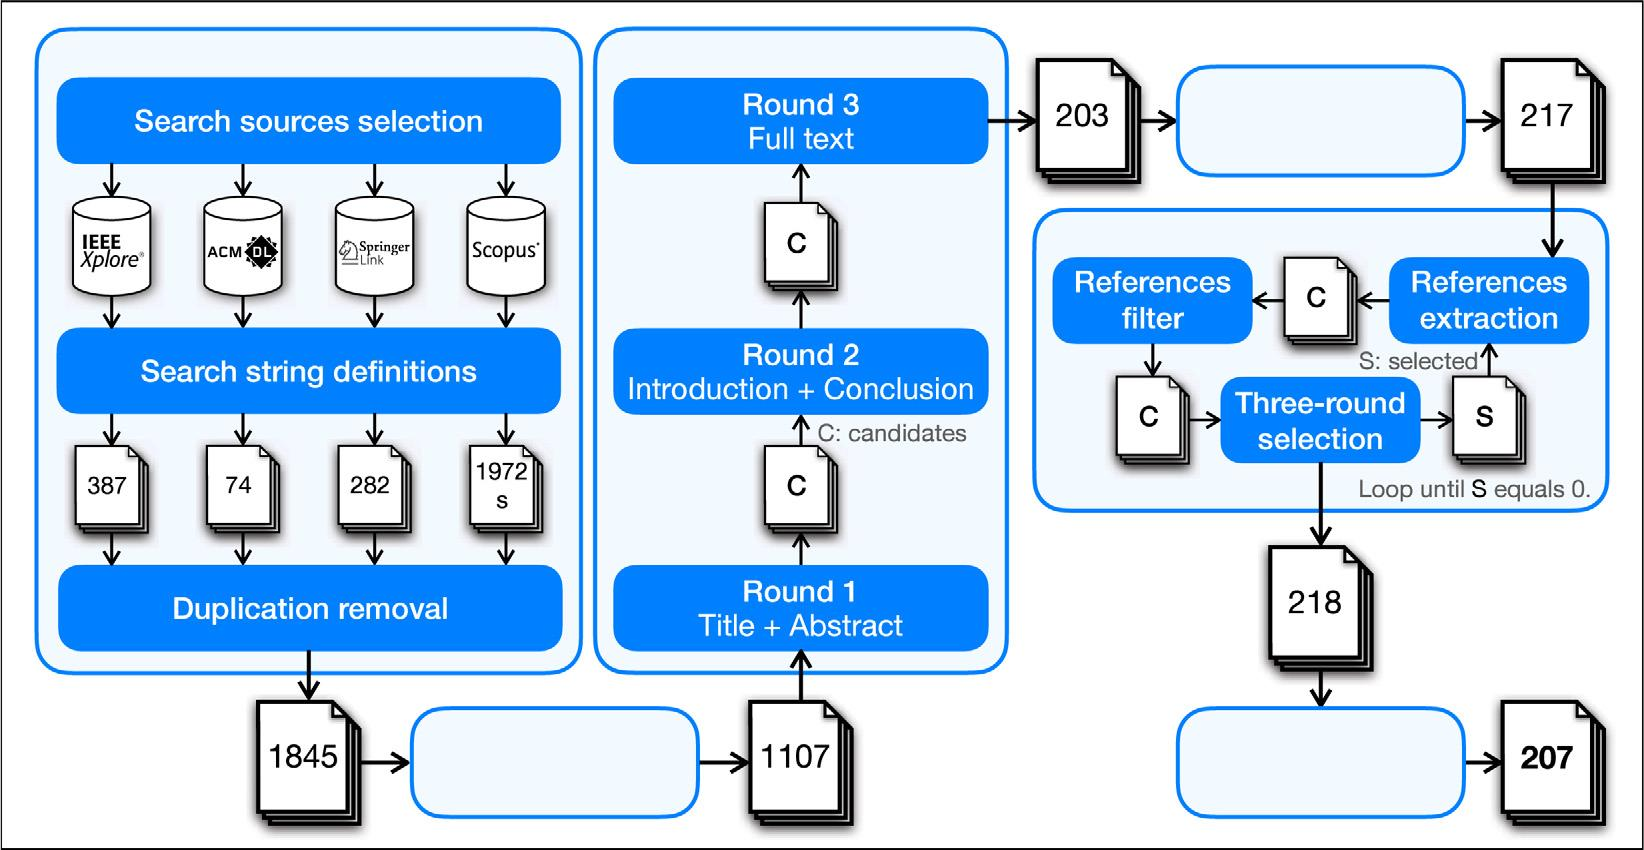
\includegraphics[width=0.9\textwidth]{Image/fig-1.jpg}
                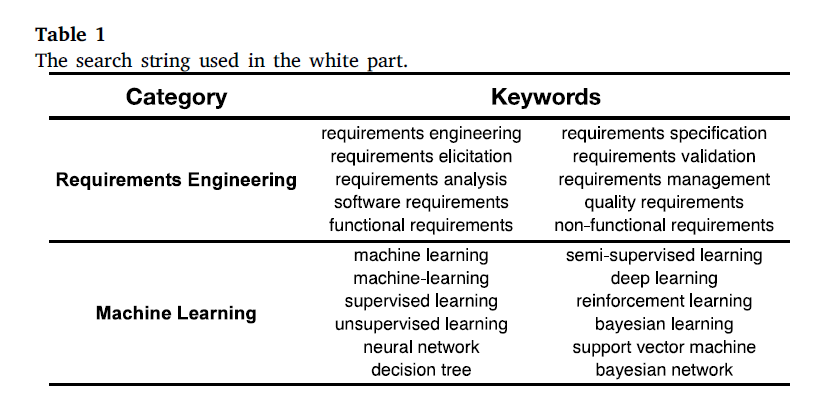
\includegraphics[width=0.9\textwidth]{Image/table-1.png}
            \end{figure}

            \subsubsection{جستجوی سیستماتیک}

                ما جستجوی سیستماتیک بخش سفید خود را با استفاده از رشته جستجوی پیش‌تعریف شده در چهار پایگاه داده علمی انجام می‌دهیم. فرآیند جستجوی سیستماتیک در بخش سفید شامل سه مرحله است. ما هر مرحله را به ترتیبی که در شکل ۱ نشان داده شده است، توضیح می‌دهیم.

                انتخاب منابع جستجو. منابع جستجو می‌توانند به طور قابل توجهی کیفیت بررسی سیستماتیک ادبیات را تحت تأثیر قرار دهند. همانطور که توسط بسیاری از مطالعات پیشنهاد شده است [35،37]، منابع جستجو باید شامل چندین پایگاه داده معتبر باشند. به طور خاص، ما چهار پایگاه داده علمی را انتخاب کرده‌ایم: IEEE Xplore، ACM Digital Library، SpringerLink و Scopus. این چهار پایگاه داده می‌توانند بیشتر از ادبیات مرتبط با مهندسی نیازها را پوشش دهند [38].

                تعریف رشته جستجو. موضوع اصلی مطالعه ما یادگیری ماشین برای مهندسی نیازها است. ما رشته جستجو را به دو بخش تقسیم کرده‌ایم: بخش مهندسی نیازها و بخش تکنیک‌های یادگیری ماشین. این دو بخش با استفاده از عملگر 'AND' به هم متصل شده‌اند. به طور خاص، هر بخش شامل اصطلاحات کلیدی مرتبط است و اصطلاحات کلیدی در هر بخش با استفاده از عملگر 'OR' به هم متصل شده‌اند. برای اطمینان از پوشش جستجوی جامع و کاهش تلاش‌های انتخاب دستی، چندین دوره انجام شد تا کلمات کلیدی تعیین و بهبود یابند. جزئیات کامل رشته‌های جستجو در جدول ۱ توضیح داده شده است. علاوه بر این، جستجوی snowballing در بخش ۳.۲.۵ برای گسترش دامنه جستجو به کار گرفته می‌شود.

                حذف تکرار. ما برای پیدا کردن مقالاتی که عنوان، چکیده یا کلمات کلیدی آن‌ها شامل رشته جستجوی پیش‌تعریف شده در چهار پایگاه داده هستند و محدوده سال انتشار را بین سال‌های ۲۰۱۰ تا ۲۰۲۲ قرار داده‌ایم. مهم باید توجه داشت که SpringerLink فقط جستجوی متن کامل را پشتیبانی می‌کند، که نیازمند بررسی‌های اضافی در نتایج جستجوی این پایگاه داده است. به طور خاص، ما از توابع Google Sheets برای ادغام عنوان، چکیده و کلمات کلیدی هر مقاله استفاده کردیم و آن‌ها را با استفاده از عبارات منظم پیش‌تعریف شده با یکدیگر مطابقت دادیم. این فرآیند تعداد مقالات از ۷۳۶۷ مقاله در SpringerLink به ۲۸۲ مقاله کاهش داد. سپس، ما ۳۸۷ مقاله از IEEE Xplore، ۷۴ مقاله از ACM Digital Library، ۲۸۲ مقاله از SpringerLink و ۱۹۷۲ مقاله از Scopus به دست آوردیم. پس از حذف تمام تکرارها، تعداد ۱۸۴۵ مقاله باقی مانده است.
            
            \subsubsection{فیلتر سیستماتیک}

                نتایج اولیه جستجو از موتورهای جستجوی علمی شامل موارد زیادی است که نمی‌خواهیم مانند سخنرانی‌های اصلی، پوسترها یا مقالاتی که بسیار کوتاه هستند. علاوه بر این، موتورهای جستجو مختلف جستجوی ما را در مقیاس‌های مختلف انجام می‌دهند، اگرچه تلاش کرده‌ایم جستجوی ما را به فیلدهای عنوان، چکیده و کلمات کلیدی محدود کنیم. بنابراین، سه معیار پیش از حذف (PEC) تعریف می‌کنیم تا این نوع مقالات را از بین ببریم و بار کاری بعدی را کاهش دهیم. به دلیل استفاده از Google Sheets برای ثبت مقالات، این معیارهای انحصاری ساده از طریق توابع به صورت خودکار قابل اعمال هستند. ارزش ذکر دارد که برای PEC3 از تطبیق regex برای عنوان، چکیده و کلمات کلیدی هر مقاله با رشته جستجوی تعریف شده استفاده کردیم. پس از فیلترینگ سیستماتیک، 1107 مقاله باقی مانده است.

                \begin{itemize}
                    \item PEC1: طول مقاله کمتر از شش صفحه است.
                    \item PEC2: مقاله به زبان انگلیسی نیست.
                    \item PEC3: محتوای ترکیب شده عنوان، چکیده و کلمات کلیدی مقاله با رشته جستجوی تعریف شده مطابقت ندارد.
                \end{itemize}
            
            \subsubsection{انتخاب سه‌گانه}

                تمام مقالاتی که پس از فیلترینگ خودکار باقی مانده‌اند، سپس به صورت دستی بررسی می‌شوند تا از لحاظ ارتباط با موضوع مناسب بودند. معیار کلی انتخابی که ما تعریف کرده‌ایم این است که مقاله باید یک روش را پیشنهاد دهد که به طور اصلی از یادگیری ماشین برای کمک به وظایف مرتبط با مهندسی نیازها استفاده می‌کند.

                معیارهای اضافه و حذف. برای بهبود اجرای معیار انتخابی، آن را به سری معیارهای اضافه و حذف (IC و EC) که در جدول ۲ نشان داده شده است، تجزیه و تحلیل کرده‌ایم. اگر مقاله با هریک از معیارهای حذف مطابقت داشته باشد، آن را حذف می‌کنیم؛ و تنها در صورتی که تمامی معیارهای اضافه را برآورده کند، آن را در می‌آوریم.
                
                پروتکل انتخاب. دو نویسنده هر مقاله را از نظر معیارهای اضافه و حذف مورد بررسی قرار دادند. ابتدا مطالعه آزمایشی را بر روی ۴۰ مقاله به صورت تصادفی انجام دادیم. اگر نظرات مغایر وجود داشت، دو نویسنده نگرانی‌های خود را صریحاً بیان کرده و آن‌ها را حل کردند. از این مطالعه آزمایشی برای بهبود معیارهای ما استفاده کردیم و اجازه دادیم تا دو نویسنده بر جزییات عملی موافق شوند. پس از رسیدن به توافق در انتخاب مقالات، دو نویسنده مقالات باقیمانده را انتخاب کردند. اگر تضادی وجود داشت که دو نویسنده نتوانستند حل کنند، یک پژوهشگر سوم برای بررسی اضافی وارد می‌شد.
                
                فرآیند انتخاب. همانطور که در شکل ۱ نشان داده شده است، ما فرآیند بازبینی دستی را به سه دور تقسیم کرده‌ایم. در دور ۱، بازبینان فقط عنوان و چکیده هر مقاله را می‌خوانند تا تصمیم بگیرند که آن را حذف یا حفظ کنند. تمام مقالات باقیمانده را به دور بعد منتقل می‌کنیم. در دور ۲، بازبینان هم عنوان و هم چکیده، مقدمه و نتیجه‌گیری هر مقاله را می‌خوانند. همانطور که قبلاً بود، این مقالات را تا دور بعد حفظ می‌کنیم، به جز مقالاتی که حذف شده‌اند. در دور ۳، بازبینان نیاز دارند که متن کامل را بخوانند و سپس تصمیم نهایی را بگیرند. پس از انجام سه دور انتخاب دستی، ما ۲۰۳ مقاله را انتخاب کردیم.
            
            \subsubsection{افزایش دانش حوزه}

                در سال‌های اخیر، یادگیری ماشین به عنوان یک تکنیک گسترده، کاربردهای فراوانی در مهندسی نیازها داشته است. در طول این سال‌ها، تمرکز تحقیقات ما بر روی حوزه یادگیری ماشین برای مهندسی نیازها بوده است. به طور خاص، ما مقالات مربوطه را از جلسات معمولی مهندسی نیازها از جمله مجلات RE، REJ، REFSQ و AIRE از سال 2010 به بعد جمع‌آوری و خلاصه نموده‌ایم. ما این مقالات را از بین 1845 مقاله انتخاب نموده و به یک فرآیند انتخاب سه مرحله‌ای تحت آنها تحت‌پرسی کرده‌ایم. پس از این مرحله، ما مجموعاً 217 مقاله را جمع‌آوری کرده‌ایم، که شامل 14 مقاله جدید است.

                \begin{figure}
                    \centering
                    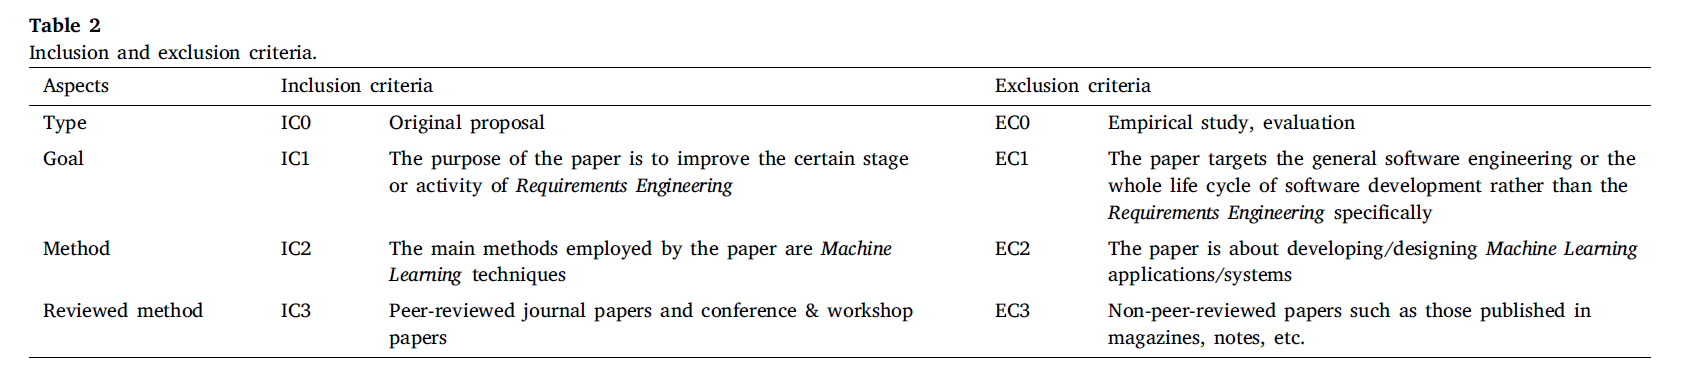
\includegraphics[width=0.9\textwidth]{Image/table-2.png}
                \end{figure}
            
            \subsubsection{جستجوی برفی}

                برای افزایش جامعیت مطالعه خود، ما جستجوی برفی را با اسکن مراجع مقالات انتخاب شده از طریق روش قبلی انجام دادیم.

                استخراج مراجع: ما حدود ۹۰۰۰ مرجع را از تمامی ۲۱۷ مقاله در اولین دور جستجوی برفی خود استخراج کردیم.
                
                فیلتر مراجع: ابتدا ما به صورت خودکار و سیستماتیک ۹۰۰۰ مرجع را فیلتر کردیم. به طور خاص، ما مراجعی را که با رشته جستجوی مشخص شده در جدول ۱ همخوانی داشتند را انتخاب کردیم. پس از آن، ۲۴۴ مرجع انتخاب شد. پیش از استخراج عنوان مقالات از این مراجع به صورت دستی، تمامی مقالات قبل از سال ۲۰۱۰ و کمتر از شش صفحه را حذف کردیم. سپس مراجع تکراری را حذف نمودیم و ۱۰ مورد یکتا به عنوان نامزدهای مراحل بعدی باقی ماندند.
                
                انتخاب سه مرحله‌ای: این روند انتخاب سه مرحله‌ای همانند بخش ۳.۲.۳ است. پس از سه مرحله انتخاب، یک مقاله به تنهایی انتخاب شد و جستجوی برفی مکرر در این مقاله هیچ مقاله جدیدی تولید نکرد. به عبارت دیگر، پس از جستجوی برفی، ما به جمع کل ۲۱۸ مقاله رسیدیم.
            
            \subsubsection{شناسایی و فیلتر کارهای گسترده‌تر}

                ما متوجه شدیم که در 218 مقاله، 11 جفت ارتباط گسترده‌تری دارند. ما مقالات گسترده‌تر را به عنوان نتیجه‌ای از این کارهای تحقیقاتی در نظر گرفتیم. بنابراین، مقالات قبل از گسترش را از مجموعه ما حذف کردیم. در نهایت، در بخش سفید، مجموعه داده نهایی ما شامل 207 مقاله است. ما این مقالات را با شماره‌های آنها در تحلیل بعدی شناسایی می‌کنیم.
        
        \subsection{فرایند انتخاب بخش خاکستری}

            شکل ۲ روند فرآیند انتخاب در بخش خاکستری را نشان می‌دهد و تعداد سوال‌های به دست آمده در هر مرحله نیز در شکل قید شده است. در زیربخش‌های بعدی جزئیات هر یک از این مراحل آورده شده است.
        
                \subsubsection{انتخاب منبع جستجو}

                    بر اساس دسته‌بندی گاروسی و همکاران [39]، Stack Overflow به عنوان یک منبع ادبیات خاکستری از رده دوم با اعتبار متوسط در نظر گرفته می‌شود که امکان تحلیل کمّی را فراهم می‌آورد. ما Stack Overflow را به عنوان منبع داده در بخش خاکستری انتخاب کردیم به دلیل طبیعت قابل دسترس و قابل تحلیل آن.

                    \begin{figure}
                        \centering
                        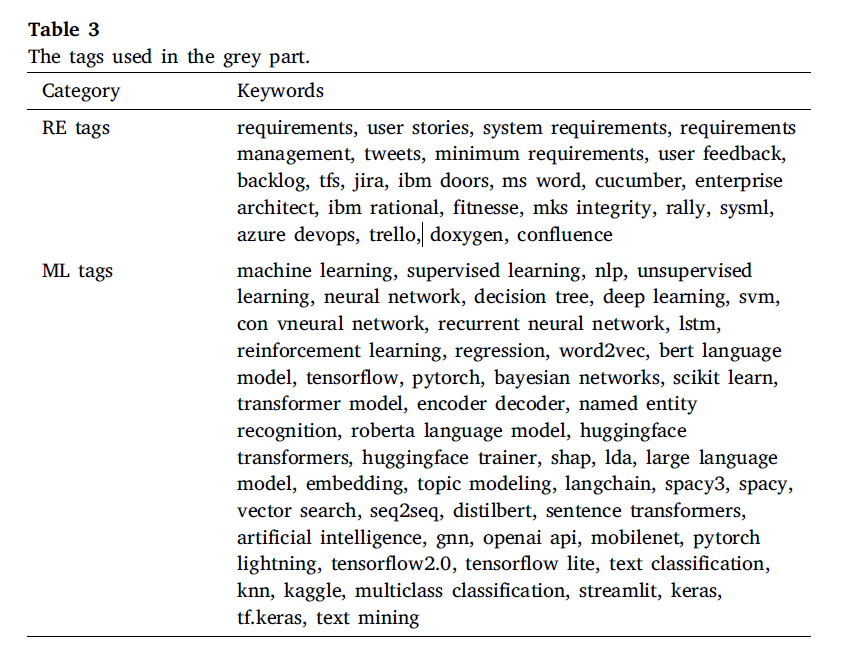
\includegraphics[width=0.9\textwidth]{Image/table-3.png}
                    \end{figure}

                \subsubsection{فیلترینگ بر اساس برچسب‌ها}
                    ما مجموعاً 23,758,292 سوال در Stack Overflow پیدا کردیم. برای شناسایی و فیلتر کردن سوال‌های مرتبط با مهندسی نیازمندی‌ها، از برچسب‌ها به عنوان ابزارهای دسته‌بندی استفاده کردیم. به طور خاص، شش برچسب زیر را انتخاب کردیم: requirements، user-stories، system-requirements، requirements-management، minimum-requirements، و REtags and MLtags که جزئیات محتوای REtags و MLtags در جدول ۳ ذکر شده است. سپس از API Stack Overflow استفاده کردیم تا تمام سوالاتی که دارای هر کدام از این برچسب‌ها از سال ۲۰۱۰ تا ۲۰۲۲ بودند، استخراج کنیم. این تلاش به تعداد سوال‌های متناظر زیر منجر شد: ۵۳۰، ۱۸۳، ۶۲، ۳۱، ۲۲ و ۷۶.

                    حذف تکرار: در Stack Overflow، سوالات ممکن است با چندین برچسب مرتبط باشند و ممکن است بیش از یکی از برچسب‌های انتخاب شده ما را شامل شوند. پس از حذف تکرارها، تعداد ۸۶۱ سوال باقی مانده است.

                \subsubsection{انتخاب دستی}

                    تمرکز ما بر روی چالش‌های عملی مواجهه شده در مهندسی نیازمندی‌ها و استخراج نیازمندی‌های عملی از آن‌ها است. بنابراین، تمامی 861 سوال که با موفقیت از فیلتر کردن بر اساس برچسب‌ها گذر کرده‌اند، به صورت دستی بررسی شده‌اند از نظر ارتباط با مهندسی نیازمندی‌ها. دو نویسنده هر سوال را بر اساس معیار انتخابی ارزیابی کرده‌اند. یک مطالعه پیلوت اولیه شامل ۵۰ سوال به صورت تصادفی انتخاب شده انجام شد تا نظرات متضاد را مورد بررسی قرار دهد و به نویسندگان کمک کند تا به توافق برسند. سپس، دو نویسنده سایر سوالات را ارزیابی کردند. در نهایت، 375 سوال برای بخش خاکستری انتخاب شدند.
        
        \subsection{استخراج داده و ترکیب آنها}

            این بخش شرح فرآیندهای استخراج داده و سنتز آنها برای بخش‌های سفید، خاکستری و مشترک را ارائه می‌دهد. ما یک مجموعه از برچسب‌ها را شناسایی کردیم که اطلاعاتی که باید از نتایج جستجو استخراج شود به عنوان معیارها عمل می‌کنند، با هدف پاسخگویی به سوالات تحقیقاتی براساس اطلاعات به دست آمده.

            
            \begin{figure}
                \centering
                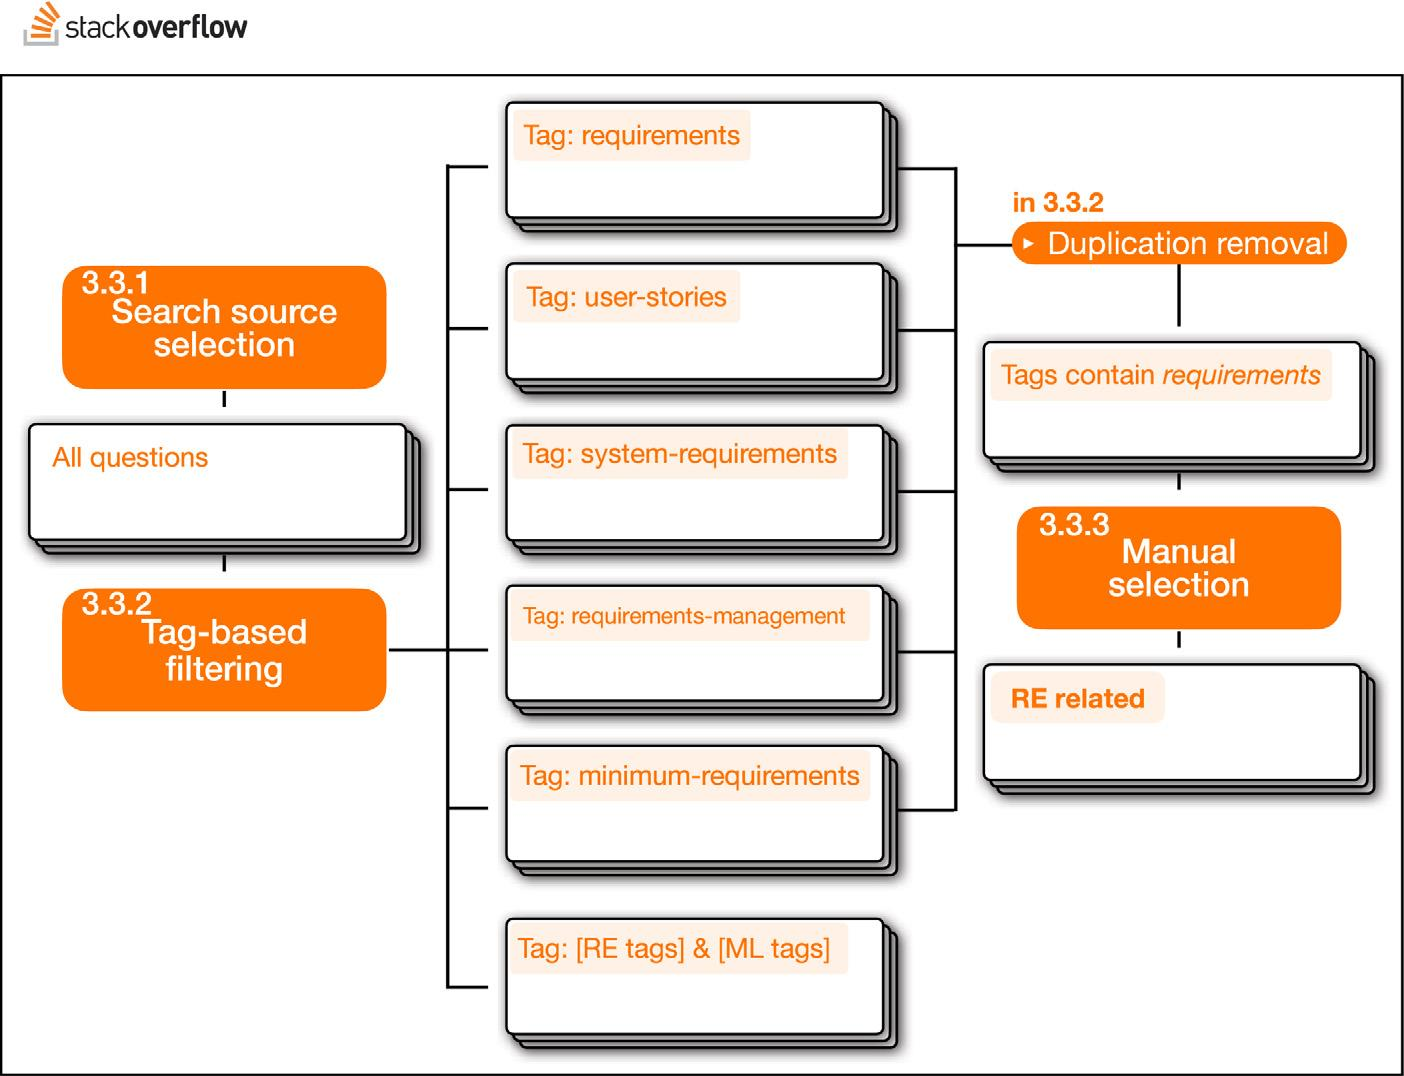
\includegraphics[width=0.9\textwidth]{Image/fig-2.jpg}
            \end{figure}

                \subsubsection{استخراج و ترکیب داده‌های سفید}

                    برای پاسخ به سوال تحقیق شماره ۱ (RQ1)، قصد داریم چهار جنبه اطلاعات را از مقالات استخراج کنیم که هرکدام شامل مجموعه‌ای از برچسب‌ها است که در شکل ۳ نشان داده شده است. توضیحات این چهار جنبه و برچسب‌های مربوط به آنها به شرح زیر است:

                    \begin{enumerate}
                        \item اطلاعات اولیه
                        \begin{enumerate}
                            \item این جنبه به درک وضعیت ابتدایی مقالات می‌پردازد و شامل چهار برچسب زیر است:
                            \begin{enumerate}
                                \item سال‌های انتشار
                                \item انواع انتشارات
                                \item محل‌های انتشار
                                \item ارجاعات (Citations)
                            \end{enumerate}
                        \end{enumerate}
                        
                        \item حوزه مسئله:
                        \begin{itemize}
                            \item این جنبه به درک تمرکز جامعه علمی بر مهندسی نیازمندی‌ها می‌پردازد و شامل دو برچسب زیر است:
                            \begin{itemize}
                                \item فعالیت‌های مهندسی نیازمندی‌ها (RE activities)
                                \item وظایف مهندسی نیازمندی‌ها (RE tasks). برای فعالیت‌های مهندسی نیازمندی‌ها، مطابق با دانش نرم‌افزاری (SWEBOK)، هر مقاله را به یکی از پنج فعالیت زیر دسته‌بندی می‌کنیم: استخراج نیازمندی‌ها، تجزیه و تحلیل نیازمندی‌ها، مشخصه‌سازی نیازمندی‌ها، اعتبارسنجی نیازمندی‌ها و مدیریت نیازمندی‌ها. برای وظایف مهندسی نیازمندی‌ها، وظایف خاص مهندسی نیازمندی‌ها از هر مقاله استخراج می‌شود بر اساس توضیحات آن.
                            \end{itemize}
                        \end{itemize}
                        
                        \item حوزه راه‌حل:
                        \begin{itemize}
                            \item این جنبه به بررسی استفاده از روش‌های یادگیری ماشین در ML4RE (یادگیری ماشین برای مهندسی نیازمندی‌ها) می‌پردازد و شامل سه برچسب زیر است:
                            \begin{itemize}
                                \item وظایف ML (ML tasks)
                                \item تکنیک‌های ML (ML techniques)
                                \item ابزارهای ML (ML tools). برای وظایف ML، انواع وظایف ML از هر مقاله استخراج می‌شود مانند طبقه‌بندی و خوشه‌بندی. سپس، تکنیک‌ها و ابزارهای خاص ML استخراج می‌شود که در هر مقاله استفاده شده‌اند. برای قابلیت تکرار، انواع مواد قابل تکرار ارائه شده در هر مقاله مانند داده، کدهای مدل و نمایش‌های آزمایش ثبت می‌شود.
                            \end{itemize}
                        \end{itemize}
                        
                        \item داده:
                        \begin{itemize}
                            \item این جنبه به مطالعه داده‌های تجزیه و تحلیل شده در ML4RE می‌پردازد و شامل دو برچسب زیر است:
                            \begin{itemize}
                                \item انواع داده‌ها (Data types)
                                \item منابع داده (Data sources). برای انواع داده‌ها، ابتدا داده‌ها را به چهار نوع عمومی دسته‌بندی می‌کنیم و سپس داده‌های خاص بر اساس محتوای مقاله ثبت می‌شود. چهار نوع عمومی داده عبارتند از: آثار نیازمندی، نظرات کاربران، داده‌های دامنه و آثار در مهندسی نرم‌افزار (SE). برای منابع داده، آنها را به یکی از پنج دسته زیر دسته‌بندی می‌کنیم: عمومی، به دست آمده، خصوصی، اصلی و بدون ذکر. همچنین، منابع داده خاص استخراج می‌شود.
                            \end{itemize}
                        \end{itemize}
                        
                        \item مدل:
                        \begin{itemize}
                            \item این جنبه به بررسی مدل‌های استفاده شده در ML4RE می‌پردازد و شامل دو برچسب زیر است:
                            \begin{itemize}
                                \item انواع مدل‌ها (Model types)
                                \item روش‌های ارزیابی مدل‌ها (Model evaluation methods). برای انواع مدل‌ها، انواع مدل‌های استفاده شده در هر مقاله مانند شبکه‌های عصبی مصنوعی، درخت تصمیم، رگرسیون و ... ثبت می‌شود. برای روش‌های ارزیابی مدل‌ها، روش‌های مختلفی مانند دقت، بازخوانی، دقت و بازخوانی متوازن، ماتریس درهم‌ریختگی و ... مورد بررسی قرار می‌گیرد.
                            \end{itemize}
                        \end{itemize}
                    \end{enumerate}
                    

                    این جنبه‌ها و برچسب‌ها به عنوان معیارها برای تجزیه و تحلیل سیستماتیک اطلاعات به دست آمده از مقالات استفاده می‌شوند تا به پاسخگویی به سوالات تحقیقی بپردازیم.


                    \begin{figure}
                        \centering
                        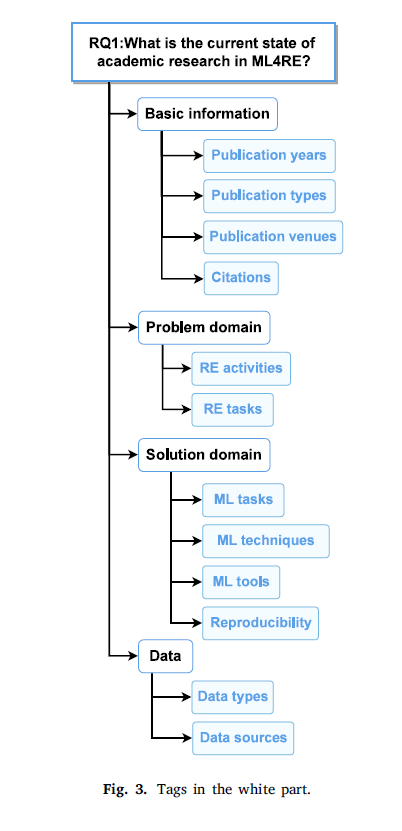
\includegraphics[width=0.5\textwidth]{Image/fig-3.jpg}
                    \end{figure}

                \subsubsection{استخراج و سنتز داده‌های خاکستری}

                    برای پاسخ به سوال تحقیق شماره ۲ (RQ2)، طراحی شده است که چهار جنبه اطلاعات را از سوالات و پاسخ‌ها استخراج کنیم، هرکدام شامل مجموعه‌ای از برچسب‌ها هستند که در شکل ۴ نشان داده شده است. توضیحات این چهار جنبه و برچسب‌های مربوط به آنها به شرح زیر است:

                    \begin{enumerate}
                        \item اطلاعات اولیه:
                        \begin{itemize}
                            \item این جنبه به درک وضعیت ابتدایی سوالات می‌پردازد، شامل چهار برچسب زیر است:
                            \begin{itemize}
                                \item سال‌های ارسال
                                \item انواع سوالات
                                \item وضعیت سوال
                                \item تعداد پاسخ‌ها. برای انواع سوالات، بر اساس محتوا، سوالات را به پنج نوع دسته‌بندی می‌کنیم: تعریف‌های مفهومی، روش‌های عملی در عمل، مشکلات خاص در عمل مهندسی نیازمندی‌ها، مشکلات در استفاده از ابزار و نیاز به راه‌حل‌ها. برای وضعیت سوال، ثبت می‌کنیم که آیا پرسش کننده سوال پاسخ را قبول کرده است یا خیر.
                            \end{itemize}
                        \end{itemize}
                        
                        \item حوزه مسئله:
                        \begin{itemize}
                            \item این جنبه به مطالعه چالش‌های عملی مهندسی نیازمندی‌ها که در جامعه Stack Overflow مواجه می‌شوند می‌پردازد، شامل دو برچسب زیر است:
                            \begin{itemize}
                                \item فعالیت‌های مهندسی نیازمندی‌ها (RE activities)
                                \item وظایف مهندسی نیازمندی‌ها (RE tasks). مشابه بخش سفید، هر سوال را بر اساس SWEBOK به یکی از پنج فعالیت مهندسی نیازمندی‌ها دسته‌بندی می‌کنیم. علاوه بر این، وظایف شناسایی شده در بخش سفید را در زمان تعیین وظایف RE به سوالات در نظر می‌گیریم.
                            \end{itemize}
                        \end{itemize}
                        
                        \item حوزه راه‌حل:
                        \begin{itemize}
                            \item این جنبه به بررسی استفاده از ابزارها در جامعه Stack Overflow می‌پردازد، شامل دو برچسب زیر است:
                            \begin{itemize}
                                \item ابزارها (Tools)
                                \item یادگیری ماشین (ML). ما ابزارهای مهندسی نیازمندی‌ها مطرح شده در سوالات و پاسخ‌ها را جداگانه ثبت می‌کنیم. برای ML، اطلاعات مربوط به ML را بر اساس فرآیند در بخش سفید استخراج می‌کنیم.
                            \end{itemize}
                        \end{itemize}
                        
                        \item داده:
                        \begin{itemize}
                            \item این جنبه به مطالعه داده‌های تجزیه و تحلیل شده در جامعه Stack Overflow می‌پردازد، شامل تنها یک برچسب زیر است:
                            \begin{itemize}
                                \item انواع داده‌ها (Data types). ابتدا انواع خاص داده‌های پردازش شده در هر سوال را ثبت می‌کنیم. سپس، همه انواع داده‌های خاص را به دسته‌های داده‌های کلی‌تری که در بخش سفید استفاده شده‌اند، گروه‌بندی می‌کنیم.
                            \end{itemize}
                        \end{itemize}
                    \end{enumerate}

                    \begin{figure}
                        \centering
                        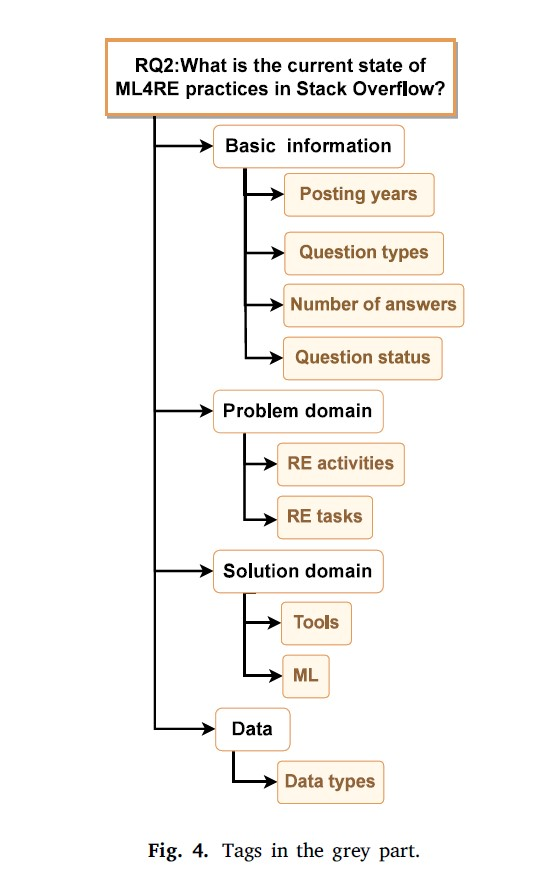
\includegraphics[width=0.5\textwidth]{Image/fig-4.jpg}
                    \end{figure}
                
            
            \subsubsection{ترکیب و تحلیل داده‌ها به صورت مشترک}

                برای پاسخ به سوال تحقیق شماره ۳ (RQ3)، قصد داریم چهار جنبه اطلاعات را از بخش سفید و بخش خاکستری مقایسه کنیم، هرکدام شامل مجموعه‌ای از برچسب‌ها که در شکل ۵ نشان داده شده است. توضیحات این چهار جنبه و برچسب‌های مربوط به آنها به شرح زیر است:

                \begin{enumerate}
                    \item اطلاعات اولیه:
                    \begin{itemize}
                        \item این جنبه برای مقایسه وضعیت ابتدایی بین تحقیقات علمی و کاربردهای عملی در Stack Overflow طراحی شده است، شامل یک برچسب زیر است:
                        \begin{itemize}
                            \item Trend (روند). به طور خاص، روند برای تمایز دادن تمرکز دانشگاهی و عملیاتی در Stack Overflow با مقایسه سال‌های انتشار در بخش سفید و سال‌های ارسال در بخش خاکستری مورد استفاده قرار می‌گیرد.
                        \end{itemize}
                    \end{itemize}
                    
                    \item حوزه مسئله:
                    \begin{itemize}
                        \item این جنبه برای مقایسه تاکید بر مهندسی نیازمندی‌ها بین دو بخش طراحی شده است، شامل دو برچسب زیر است:
                        \begin{itemize}
                            \item فعالیت‌های مهندسی نیازمندی‌ها (RE activities)
                            \item وظایف مهندسی نیازمندی‌ها (RE tasks). ما مقایسه‌ای بر اساس فعالیت‌های وظایف RE استخراج شده در بخش سفید و خاکستری انجام می‌دهیم.
                        \end{itemize}
                    \end{itemize}
                    
                    \item حوزه راه‌حل:
                    \begin{itemize}
                        \item این جنبه برای مقایسه روش‌های استفاده شده توسط دانشگاه و عملیات در Stack Overflow در حل مشکلات مهندسی نیازمندی‌ها طراحی شده است، شامل یک برچسب زیر است:
                        \begin{itemize}
                            \item ابزارها و ML (Tools\&ML). ما این مقایسه را بر اساس تکنیک‌های ML استخراج شده در بخش سفید در مقابل ابزارها و ML در بخش خاکستری انجام می‌دهیم.
                        \end{itemize}
                    \end{itemize}
                    
                    \item داده:
                    \begin{itemize}
                        \item این جنبه برای مقایسه داده‌های مورد بررسی در تحقیقات علمی با انواع داده‌های مورد بحث و تجزیه و تحلیل در جامعه Stack Overflow طراحی شده است، شامل یک برچسب زیر است:
                        \begin{itemize}
                            \item انواع داده‌ها (Data types). مقایسه بر اساس انواع داده استخراج شده در بخش سفید و خاکستری صورت می‌پذیرد.
                        \end{itemize}
                    \end{itemize}
                \end{enumerate}
                

                مانند انتخاب دستی قبلی، دو پژوهشگر برای هر مقاله به منظور انجام پردازش داده تعیین شده‌اند تا اعتبار پژوهش‌ها تضمین شود.

                \begin{figure}
                    \centering
                    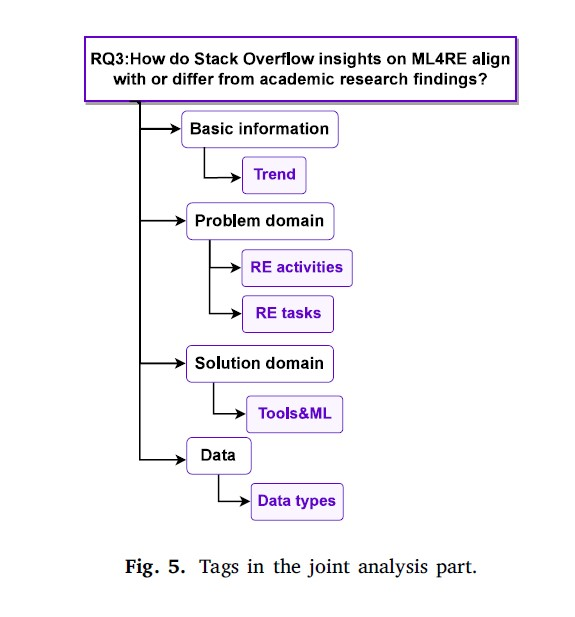
\includegraphics[width=0.5\textwidth]{Image/fig-5.jpg}
                \end{figure}
            
    % MARK: White part results (RQ1)

    \section{نتایج بخش سفید (RQ1)}

        با پیروی از طراحی در بخش 3.4.1، اطلاعات استخراج شده از مقالات برای پاسخ به سوال پژوهشی 1 (RQ1) را با برخی از نمودارهای دقیقاً طراحی شده، همانطور که در منبع [37] توصیه شده است، ارائه می‌دهیم.

        \subsection{اطلاعات پایه}

            در این زیر بخش، ما برخی اطلاعات پایه را برای درک وضعیت در جامعه علمی ارائه می‌دهیم.
        
            \subsubsection{سال‌های انتشار}
            
                در بخش سفید، ما ۲۰۷ مقاله را انتخاب کرده‌ایم. شکل ۶ تعداد مقالات در مورد ML4RE را در هر سال از ۲۰۱۰ تا ۲۰۲۲ نشان می‌دهد. همانطور که در شکل می‌بینیم، تحقیقات در این زمینه طی دهه گذشته به صورت تابع درجه دوم رشد کرده است و تعداد مقالات از سال ۲۰۱۶ به طور قابل توجهی افزایش یافته است. برای تسهیل بحث‌های بعدی، ما به طور موقت ۱۳ سال گذشته را به دو مرحله تقسیم می‌کنیم: مرحله اولیه (۲۰۱۰–۲۰۱۵) و مرحله توسعه (۲۰۱۶–۲۰۲۲).

            \subsubsection{انواع انتشارات}

                در مقالاتی که انتخاب کرده‌ایم، 115 مقاله کنفرانس، 66 مقاله ژورنال و 26 مقاله کارگاهی وجود دارد. تعداد هر نوع مقاله در هر سال در شکل 7 است. به طور خاص، تعداد مقالات کنفرانسی در چهار سال اول(2016-2019) پس از ورود به فاز توسعه، به سرعت افزایش یافت. با گذشت زمان و تجمع کارهای تحقیقاتی، تعداد مقالات ژورنالی از سال 2020 آغاز به افزایش یافت. در پنج سال قبل از سال 2020، میانگین تعداد مقالات ژورنالی تنها 4.6 مقاله بر سال بود. با این حال، تنها در سال 2020، 13 مقاله ژورنالی در این حوزه منتشر شد. در سال 2022، آن‌ها 17 مقاله ژورنالی منتشر کردند و به اوج جدیدی رسیدند.

                \begin{figure}
                    \centering
                    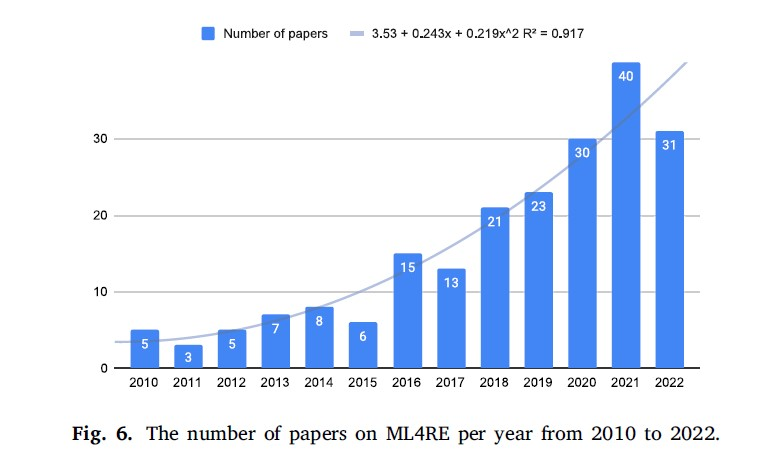
\includegraphics[width=0.5\textwidth]{Image/fig-6.jpg}
                    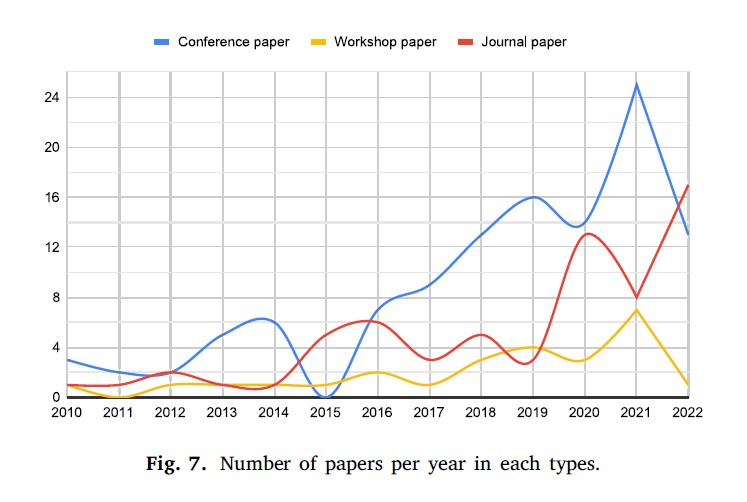
\includegraphics[width=0.5\textwidth]{Image/fig-7.jpg}
                \end{figure}


            \subsubsection{محل‌های انتشار}

            
                پژوهشگران ۲۰۷ مقاله را که انتخاب کرده‌ایم، در ۱۲۹ محل انتشار منتشر کردند. جدول ۴، مروری از محل‌های انتشار را نشان می‌دهد، با دسته‌بندی محل‌هایی که تنها یکبار ظاهر شده‌اند به عنوان محل‌های دیگر. همان‌طور که جدول ۴ نشان می‌دهد، ۲۴ محل با چندین انتشار تقریباً نصف مقالات (۱۰۲ از ۲۰۷، ۴۹.۳٪) را منتشر کرده‌اند. آن‌ها تقریباً همهٔ محل‌های کلاسیک در جامعهٔ توسعه الزامات هستند. مابقی ۱۰۵ مقاله در محل‌های گسترده‌ای ظاهر شده‌اند (۱۰۵ از ۲۰۷، ۵۰.۷٪) که به اشتراک گذاری ML4RE را بیرون از اجتماع توسعه الزامات کمک می‌کند. در نظرسنجی ما، متوجه شدیم که ۱۶ مقاله به روابط گسترده اشاره دارند. جدول ۵ اطلاعات مربوط به این ۱۶ جفت مقاله با روابط گسترده را نشان می‌دهد. بیشتر آن‌ها مواردی هستند که یک مقالهٔ کنفرانسی به یک مقالهٔ ژورنالی گسترده شده است. به عنوان مثال، پنج مقالهٔ ژورنالی از مقاله‌های کنفرانسی در سال ۲۰۲۰ گسترش یافتند. این نتیجه بیشتر نشان می‌دهد که مقالات ژورنال از تجمیع کارهای پژوهشی پیشین در زمینهٔ ML4RE ناشی می‌شوند.
            
            \subsubsection{نقل قول‌ها}

                ما روابط نقل قول بین مقاله‌های انتخابی را مستند کرده‌ایم، فراوانی هر مقاله که توسط کارهای دیگر انتخابی نقل قول شده است، را ثبت کرده‌ایم. در نهایت، ما مقالاتی را با بیشترین تعداد نقل قول شناسایی کرده‌ایم: P053، P002، P022، P014، P018، P040، P058، P023 و P051.

                نقل قول‌های معتبری که این مقالات به دست آوردند با نقش نماینده آن‌ها در مراحل توسعه ایجاد شده‌اند. به ویژه، P002 (۲۰۱۰) از تکنیک‌های بیزین نیو استفاده کرده است تا الزامات غیر تابعی را به صورت خودکار شناسایی و دسته‌بندی کند. مطالعات بعدی، به عنوان مثال P014، P018، P022 و P023 (۲۰۱۳-۲۰۱۴)، به بررسی عمیق‌تر از استفاده از تکنیک‌های پردازش زبان طبیعی، مانند مدل‌سازی موضوع، پرداختند. در ادامه، P040، P053، P058 و P051 (۲۰۱۶-۲۰۱۷) تمرکز خود را به بهره‌گیری از یادگیری عمیق و استخراج متن برای تحلیل خودکار مجموعه‌داده‌های بزرگ منتقل کردند. در واقع، نقل قول‌های قابل توجه این مقالات ممکن است از نقش سازنده آن‌ها در گذاشتن اساس برای تحقیقات بعدی در هر مرحله ناشی شده باشد.

                \begin{figure}
                    \centering
                    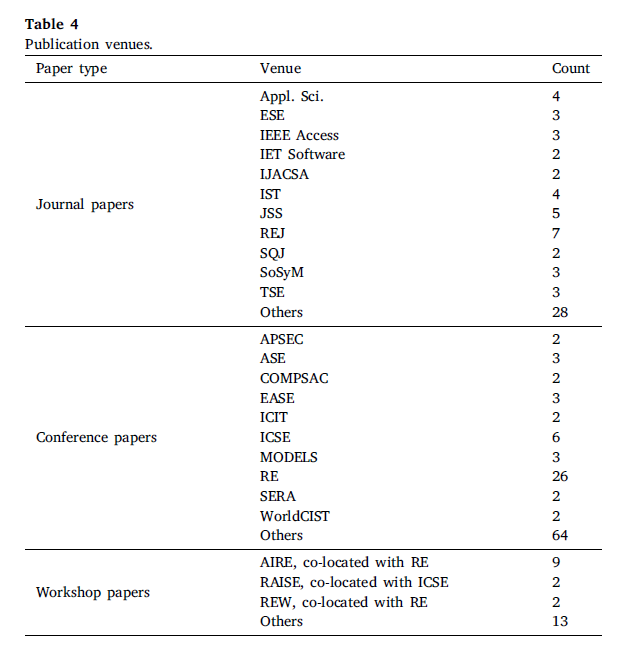
\includegraphics[width=0.5\textwidth]{Image/table-4.png}
                    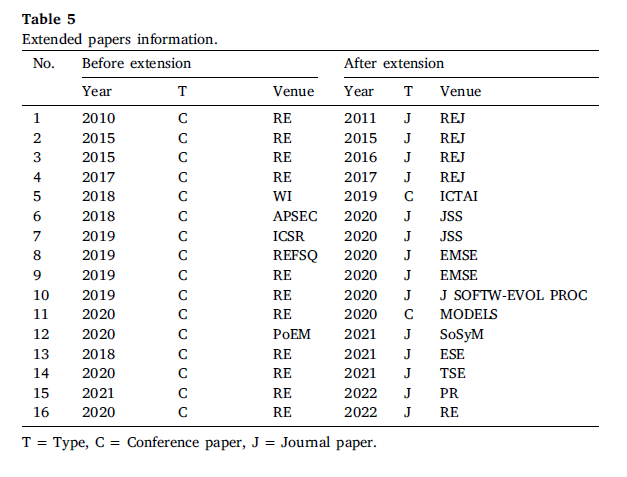
\includegraphics[width=0.5\textwidth]{Image/table-5.png}
                \end{figure}

            \subsection{حوزه‌ی مسئله}

                در این زیربخش، تمرکز جامعه‌ی علمی بر روی انجام الزامات نرم‌افزار (RE) را ارائه می‌دهیم.

            \subsubsection{فعالیت‌های RE}

                ما تعداد فعالیت‌های RE که توسط تکنیک‌های یادگیری ماشینی به آن‌ها کمک شده است، شمردیم. تجزیه و تحلیل الزامات فعالیتی است که توسط تکنیک‌های یادگیری ماشینی بیشترین حمایت را دارد با تقریباً نیمی از مقالات (90/207، 43.48\%). برای بقیه، تعدادی از جمع‌آوری و اعتبارسنجی الزامات مشابه است، 59 برای اولی و 36 برای دومی. آن‌ها در مجموع بیش از 40\% از کل 207 مقاله‌ی انتخابی را تشکیل می‌دهند. در نهایت، 22 تحقیق (10.63\%) از تکنیک‌های یادگیری ماشینی در فاز مدیریت الزامات استفاده نمودند. در مقالات انتخابی ما، هیچ تحقیقی از تکنیک‌های یادگیری ماشینی برای مشخصات الزامات استفاده نکرد.
                    
            \subsubsection{وظایف RE}

                ما فعالیت‌ها و وظایف مربوط به RE را در شکل ۸ خلاصه می‌کنیم. ۲۰۷ مقاله بر روی ۴۲ وظیفهٔ مختلف تمرکز داشتند. طبقه‌بندی نیازمندی‌ها (۴۳/۲۰۷، ۲۰.۷۷٪) پرکارترین وظیفه در طول تحلیل نیازمندی و حتی در همهٔ فعالیت‌های RE است. مدل‌سازی نیازمندی‌ها (۱۵، ۷.۲۵٪)، استخراج و طبقه‌بندی نیازمندی‌ها (۹، ۴.۳۵٪) و شناسایی نیازمندی‌ها (۶، ۲.۹۰٪) نیز وظایف پرطرفدار دیگری در فرایند تحلیل نیازمندی هستند. در مرحلهٔ جمع‌آوری، طبقه‌بندی بازخورد کاربر (۱۹، ۹.۱۸٪)، استخراج ویژگی‌ها (۱۴، ۶.۷۷٪) و استخراج نیازمندی‌ها (۱۱، ۵.۳۲٪) وظایفی هستند که بیشترین توجه را جلب کرده‌اند. ارزیابی کیفیت نیازمندی‌ها (۱۴، ۶.۷۶٪) و تشخیص ابهام در اسناد نیازمندی‌ها (۸، ۳.۸۷٪) پرطرفدارترین وظایف در طول فرآیند اعتبارسنجی نیازمندی هستند. در مدیریت نیازمندی، اولویت‌بندی نیازمندی‌ها (۹، ۴.۳۵٪) و ردیابی نیازمندی‌ها (۹، ۴.۳۵٪) متمرکز بر توجه پژوهشگران می‌باشند.

                یازده وظیفهٔ یاد شده بالا توجه بیشتری از سوی پژوهشگران در تمام مراحل RE جلب کرده‌اند. ۱۵۷ مقاله به این یازده وظیفه متناظر بوده‌اند که نمایانگر ۷۵.۸۵٪ از کل (۱۵۷/۲۰۷) است. ارزشیابی کاری‌ها نشان می‌دهد که ۵۰ مقاله با ۳۱ وظیفه پژوهشی پراکنده در مراحل مختلف مهندسی نیازمندی روبرو شده‌اند. این داده‌ها نشان می‌دهند که تعداد زیادی (۳۱/۴۲، ۷۳.۸۱٪) از وظایف RE در حوزهٔ ML4RE همچنان نیازمند بررسی بیشتر هستند.

                \begin{figure}
                    \centering
                    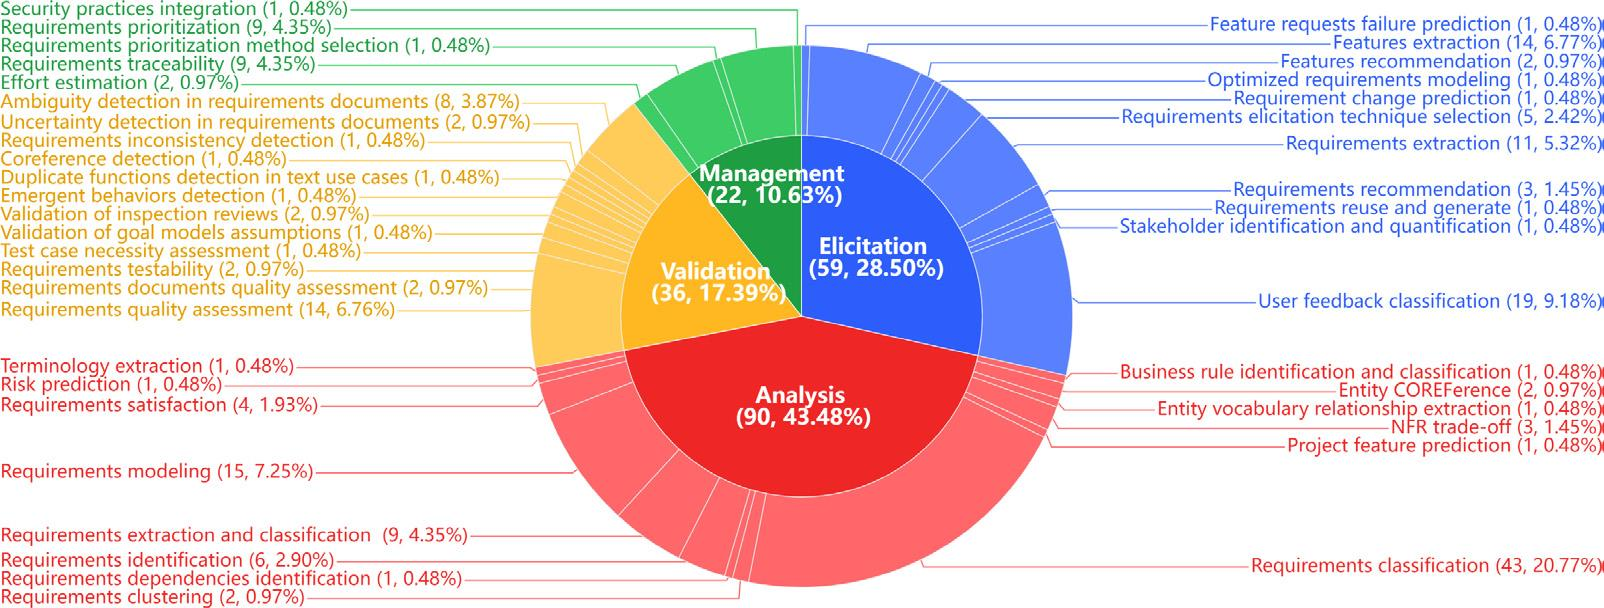
\includegraphics[width=0.5\textwidth]{Image/fig-8.jpg}
                \end{figure}

            
        \subsection{دامنه راه‌حل}
        
            در این زیربخش، ما وضعیت تکنیک‌های یادگیری ماشین مورد استفاده در حل مسائل مهندسی نیاز به نرم‌افزار ارائه می‌دهیم.

            \subsubsection{وظایف یادگیری ماشین}

                ما انواع وظایفی که تکنیک‌های یادگیری ماشین هر سال پردازش می‌کنند را شمردیم که در شکل 9 نشان داده شده است. آشکار است که طبقه‌بندی بخش قابل توجهی را تشکیل می‌دهد، در حالی که انواع دیگر وظایف سهم کمتری دارند.

            \subsubsection{تکنیک‌های یادگیری ماشین}

                در انتخاب ما از 207 مقاله، پژوهشگران 72 تکنیک یادگیری ماشین مختلف را 308 بار استفاده کردند. شکل 10 رتبه‌بندی این تکنیک‌ها بر اساس تعداد استفاده‌ها را نشان می‌دهد. ما همه 47 تکنیک یادگیری ماشین که فقط یکبار استفاده شده‌اند را به عنوان «دیگران» دسته‌بندی می‌کنیم. پراستفاده‌ترین تکنیک یادگیری ماشین SVM (37 بار استفاده شده) است، در حالی که تکنیک‌های بعدی بیشتر استفاده شده شامل CNN (20 بار)، درخت تصمیم (17 بار)، BERT (17 بار) و جنگل تصادفی (15 بار) هستند. این داده‌ها یک روند مهم در استفاده از تکنیک‌های یادگیری ماشین در مقالات یادگیری ماشین برای مهندسی نیاز به نرم‌افزار را نشان می‌دهند. استفاده بالا از روش‌های پیشرفته مانند BERT نشان دهنده تلاش مداوم پژوهشگران برای اکتشاف فناوری‌های روز دنیا است. علاوه بعد از این، از اثربخشی ادامه‌دار روش‌های سنتی یادگیری ماشین مانند Naive Bayes نشانه‌های معتبری مشخص است.
            
            \subsubsection{ابزارهای یادگیری ماشین}

                بیش از نیمی از پژوهشگران (123/207) ابزارهای یادگیری ماشینی که در مقالات خود استفاده کرده‌اند را ذکر کرده‌اند، آن‌ها 31 ابزار یادگیری ماشین را 120 بار استفاده کرده‌اند. بیشتر ابزارهای یادگیری ماشین از جمله scikit-learn، دنبال شده توسط Weka، TensorFlow، Keras، Pytorch و Matlab هستند.

                \begin{figure}
                    \centering
                    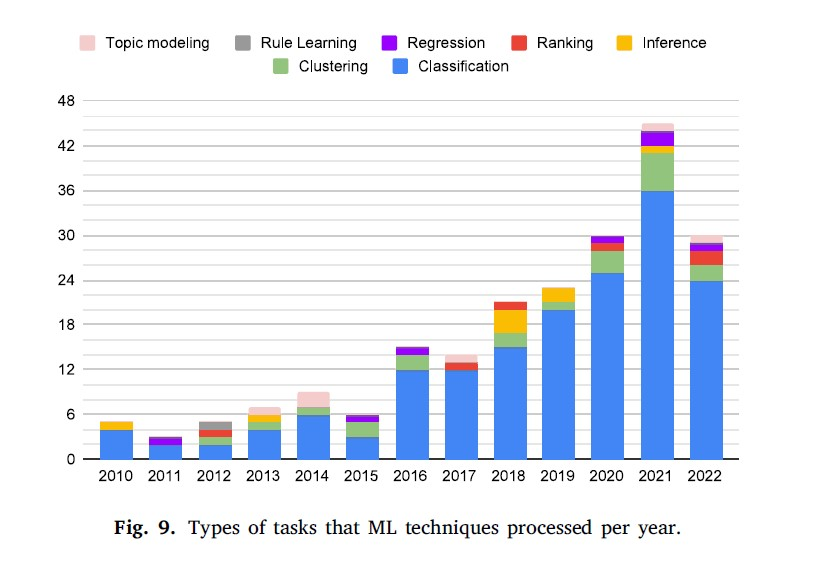
\includegraphics[width=0.5\textwidth]{Image/fig-9.jpg}
                    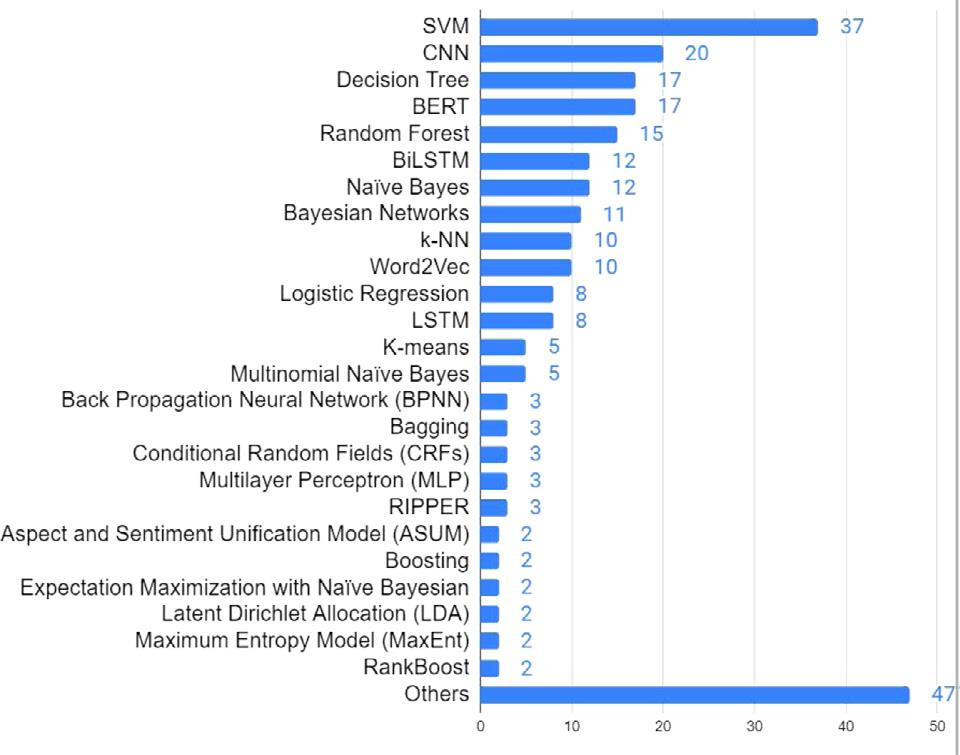
\includegraphics[width=0.5\textwidth]{Image/fig-10.jpg}
                \end{figure}
            

            \subsubsection{قابلیت تکرارپذیری}

                در زمینه بازتولید تحقیقات در حوزه ML4RE، محققان مواد را در سه جنبه ارائه می‌دهند: داده‌ها، کدهای مدل و مصنوعات تجربی. نزدیک به چهل درصد (۷۷/۲۰۷، ۳۷.۲٪) از مقالات حداقل یک ماده برای بازتولید ارائه کرده‌اند. بیشتر مواد بازتولید در داده‌ها یافت می‌شوند، پس از آن کدهای مدل و در نهایت مصنوعات تجربی. ما همچنین مواد ارائه شده در مقالات را مستند کرده‌ایم تا به محققان در دسترسی به منابع اضافی کمک کنیم.

                \begin{figure}
                    \centering
                    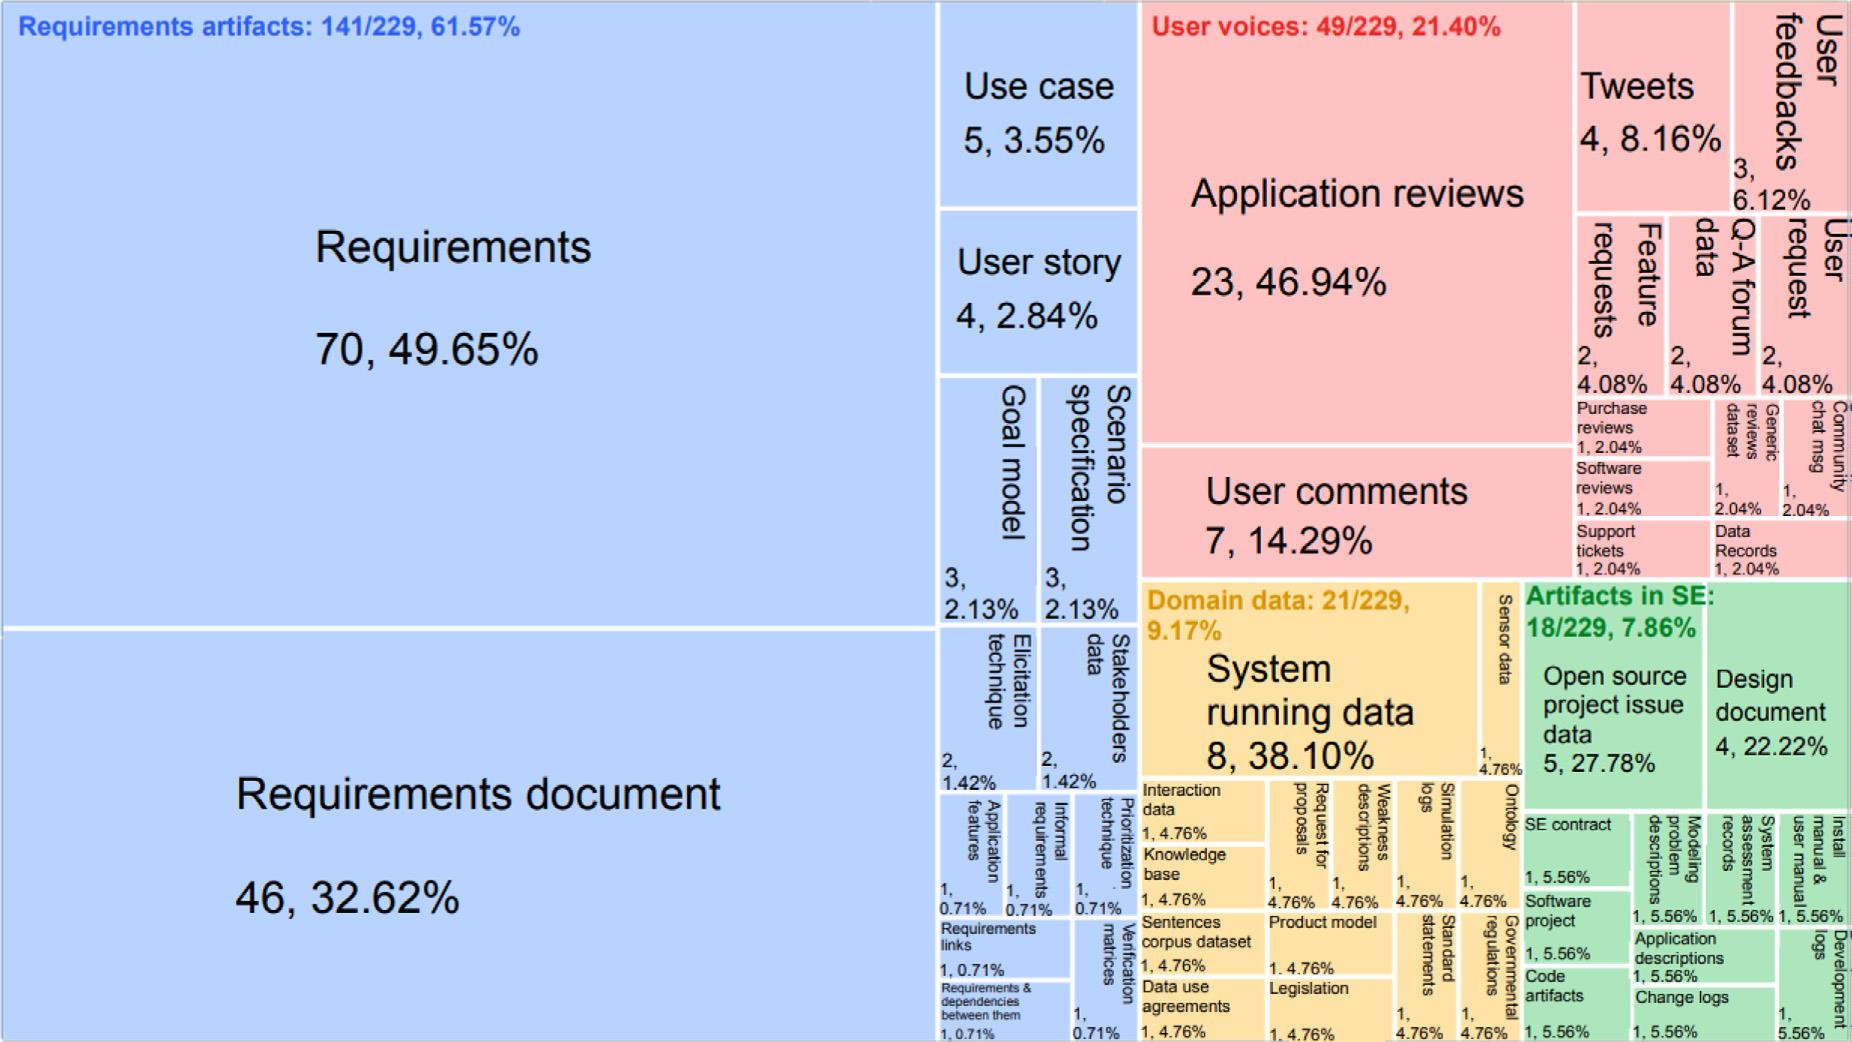
\includegraphics[width=0.5\textwidth]{Image/fig-11.jpg}
                \end{figure}

        \subsection{داده‌ها}


            در این زیر بخش، وضعیت داده‌های حوزه RE پردازش شده توسط دانشگاه‌ها را معرفی می‌کنیم.

            \subsubsection{انواع داده‌ها}

                با بررسی انواع داده‌های مورد استفاده توسط تکنیک‌های ML، ۵۳ نوع داده شناسایی شد و آنها را به چهار نوع کلی تقسیم کردیم، همانطور که در شکل ۱۱ نشان داده شده است. می‌بینیم که بیش از ۶۰٪ از داده‌ها در دسته مصنوعات نیازمندی‌ها قرار می‌گیرند، که این نوع داده‌ها بیشترین نیاز به پردازش برای حمایت از فعالیت‌ها و وظایف RE را دارند. از میان داده‌های باقی‌مانده، بیش از نیمی از آنها صدای کاربران را تشکیل می‌دهند و ۲۱.۴۰٪ از کل داده‌ها را شامل می‌شوند. این داده‌ها شامل بازخورد کاربران، درخواست‌ها و نقد و بررسی کاربران از نرم‌افزارها و برنامه‌ها، به همراه پیام‌هایی از انجمن‌های آنلاین و توییتر است. نقد و بررسی کاربران بخش عمده‌ای از صدای کاربران را تشکیل می‌دهد. داده‌های باقی‌مانده شامل مصنوعات در SE (۷.۸۶٪) و داده‌های حوزه‌ای (۹.۱۷٪) است. مصنوعات در SE شامل داده‌های چرخه حیات توسعه نرم‌افزار است. لازم به ذکر است که در اینجا مصنوعات در SE شامل مصنوعات نیازمندی‌ها نمی‌شود، زیرا آنها در دسته جداگانه‌ای به نام مصنوعات نیازمندی‌ها قرار دارند. داده‌های حوزه‌ای شامل ثروتی از دانش حوزه‌ای است و متنوع می‌باشد.

            \subsubsection{منابع داده‌ها}

                ما منابع داده‌های استفاده شده را ثبت کردیم، همانطور که در شکل ۱۲ نشان داده شده است. شانزده مقاله در مورد منبع همه یا برخی از داده‌های استفاده شده مبهم بودند و به طور صریح منبع خاص داده‌ها را ذکر نکردند. در مرحله اولیه، مقالاتی که از داده‌های عمومی استفاده می‌کردند بیشتر از مقالاتی بودند که از داده‌های منابع دیگر استفاده می‌کردند. این غلبه داده‌های عمومی در مرحله توسعه نیز مشهود است. علاوه بر این، داده‌های خزیده شده و خصوصی از سال ۲۰۱۸ به بعد روند افزایشی واضحی نشان داده‌اند.

                سپس، منبع خاص داده‌ها را به ترتیب داده‌های عمومی، خزیده شده، خصوصی و اصلی توصیف می‌کنیم.

                داده‌های عمومی. ما داده‌های عمومی را به عنوان مجموعه داده‌هایی که به طور عمومی در دسترس هستند تعریف می‌کنیم. ما دریافتیم که ۷۶ مقاله از ۴۹ منبع داده عمومی ۱۰۳ بار استفاده کرده‌اند. چندین مجموعه داده عمومی کلاسیک به طور گسترده در حوزه ML4RE استفاده شده‌اند. به عنوان مثال، مجموعه داده PROMISE در ۲۵ مقاله استفاده شده است و آن را به پرکاربردترین مجموعه داده در میان مقالات منتخب ما تبدیل کرده است. علاوه بر این، چالش داده RE17 در ۶ مقاله مورد استفاده قرار گرفته است. علاوه بر این‌ها، دیگر مجموعه داده‌های عمومی قابل توجه شامل PURE، iTrust، RE@UTS و tera-promise هستند.

                داده‌های خزیده شده. ما داده‌های خزیده شده را به عنوان داده‌هایی که از طریق خزیدن وب به دست می‌آیند مشخص می‌کنیم. رایج‌ترین مکان برای خزیدن داده، فروشگاه‌های اپلیکیشن (۱۹/۵۸، ۳۲.۸٪) است، با فروشگاه گوگل پلی و فروشگاه اپل اپ استور به عنوان منابع داده رایج. به دلیل توسعه سریع فروشگاه‌ها/بازارهای اپلیکیشن‌های موبایل، بسیاری از نقد و بررسی‌ها و توضیحات اپلیکیشن‌ها در دسترس بوده است که یکی از دلایل افزایش مقالات استفاده کننده از داده‌های خزیده شده در مرحله توسعه است.

                داده‌های خصوصی. اگر یک مقاله به صراحت ذکر کرده باشد که داده‌هایشان از پروژه‌های صنعتی واقعی یا سایر سناریوهای عملی به دست آمده است، ما منبع داده را به عنوان عملی ثبت می‌کنیم. اگر محققان بگویند که داده‌هایشان از پروژه‌ها به دست آمده است، چنین منابع داده‌ای را به عنوان نوع پروژه ثبت می‌کنیم. بر اساس تحلیل ما، ۳۷ مقاله از داده‌های عملی استفاده کرده‌اند، ۱۲ مقاله از داده‌های پروژه‌ای استفاده کرده‌اند و ۴ مقاله منبع داده‌های خود را مشخص نکرده‌اند.

                داده‌های اصلی. ما داده‌هایی که متعلق به خود محققان است را به عنوان داده‌های اصلی تعریف می‌کنیم. به طور خاص، داده‌های اصلی می‌توانند از فرآیندهای اجرای سیستم به دست آیند یا از آزمایش‌ها جمع‌آوری شوند.

                \begin{figure}
                    \centering
                    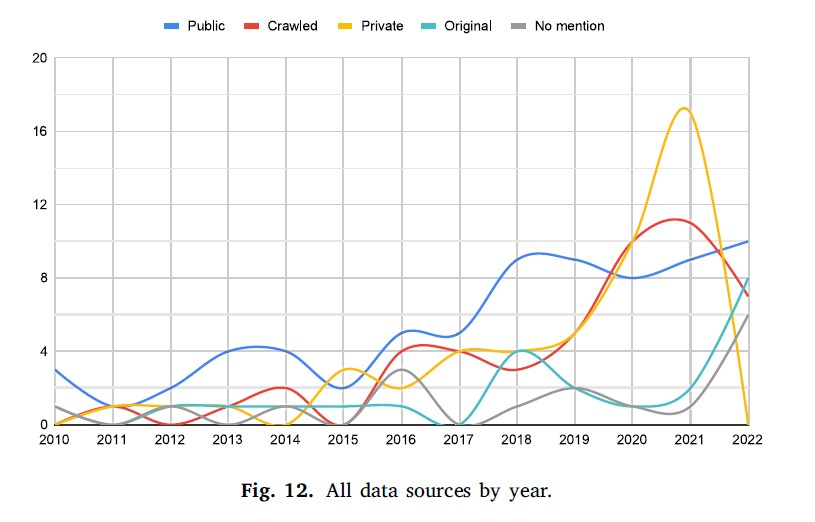
\includegraphics[width=0.5\textwidth]{Image/fig-12.jpg}
                    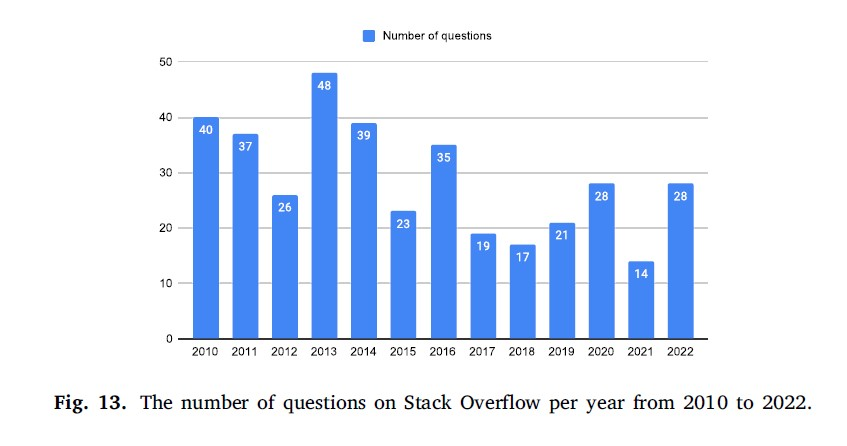
\includegraphics[width=0.5\textwidth]{Image/fig-13.jpg}
                \end{figure}

            \subsubsection{وضعیت ML4RE در دانشگاه‌ها}

                به طور خلاصه، چشم‌انداز کنونی تحقیقات ML4RE نشان‌دهنده رشد مداوم در تعداد مقالات و حرکت به سمت انتشار در مجلات با کیفیت بالاتر است. در زمینه فعالیت‌های RE، تمرکز عمده‌ای بر تحلیل RE وجود دارد و طیف گسترده‌ای از وظایف خاص مورد بررسی قرار گرفته است. علاوه بر این، تکنیک‌های ML مانند SVM، CNN، درخت‌های تصمیم‌گیری و BERT به طور گسترده‌ای استفاده می‌شوند و برخی از کارها نیز مواد حمایتی برای پروژه‌های متن‌باز ارائه می‌دهند. انواع داده‌های مورد بررسی متنوع هستند و تأکید ویژه‌ای بر مصنوعات نیازمندی‌ها دارند، و منابع عمدتاً داده‌های عمومی هستند.

    % MARK: Grey part results (RQ2)

    \section{نتایج بخش خاکستری (RQ2)}

        با پیروی از طراحی در بخش 3.4.2، اطلاعات استخراج شده از سوالات منتخب را برای پاسخ به RQ2 ارائه می‌دهیم.

        \subsection{اطلاعات پایه}

            در این زیر بخش، برخی اطلاعات پایه برای درک وضعیت در کاربردهای عملی در Stack Overflow را ارائه می‌دهیم.

            \subsubsection{سال‌های ارسال سوالات}

                پس از فرآیند جستجو و فیلتر کردن در بخش 3.3، ۳۷۵ سوال در بخش خاکستری انتخاب شد. شکل ۱۳ تعداد سوالات مرتبط با RE در Stack Overflow بین سال‌های ۲۰۱۰ تا ۲۰۲۲ را نشان می‌دهد. تعداد سوالات مرتبط با RE در Stack Overflow به طور کلی کاهش یافته است. در سال‌های ۲۰۱۰، ۲۰۱۱، ۲۰۱۳، ۲۰۱۴ و ۲۰۱۶ هر سال بیش از ۳۰ سوال وجود داشته است. از سال ۲۰۱۵ تا ۲۰۲۲، هر سال حدود ۲۰ سوال مطرح شده است.

            \subsubsection{انواع سوالات}

                بسته به محتوای سوالات، انواع سوالات را به این شکل تعریف می‌کنیم: تعاریف مفهومی، روش‌شناسی‌ها در عمل، مشکلات خاص در اجرای RE، مشکلات در استفاده از ابزارها، و نیاز به راه‌حل‌ها. نمونه سوالات این انواع در جدول ۶ نشان داده شده است. سوالات مربوط به مشکلات خاص در اجرای RE بیشترین تعداد (۳۶.۰٪) را دارند، پس از آن مشکلات در استفاده از ابزارها (۲۴.۴٪) قرار دارد. روش‌شناسی‌ها در عمل سومین دسته (۲۱.۸٪) است، در حالی که نیاز به راه‌حل‌ها ۱۰.۵٪ سوالات را تشکیل می‌دهد. تعاریف مفهومی تنها ۷.۳٪ سوالات را دارند. بر اساس محتوای سوالاتی که کاربران در Stack Overflow در مورد RE پرسیده‌اند، سه نوع سوال، تعاریف مفهومی، روش‌شناسی‌ها در عمل، و مشکلات خاص در اجرای RE، همه به دانش حوزه RE مرتبط هستند. این امر نشان می‌دهد که در کاربرد نظریه‌های RE به عمل مشکلاتی وجود دارد. از دو نوع سوال باقی‌مانده، می‌توان فهمید که کاربران در حال حاضر از چه ابزارهایی برای فعالیت‌ها، وظایف و نیازمندی‌های RE استفاده می‌کنند.

                \begin{figure}
                    \centering
                    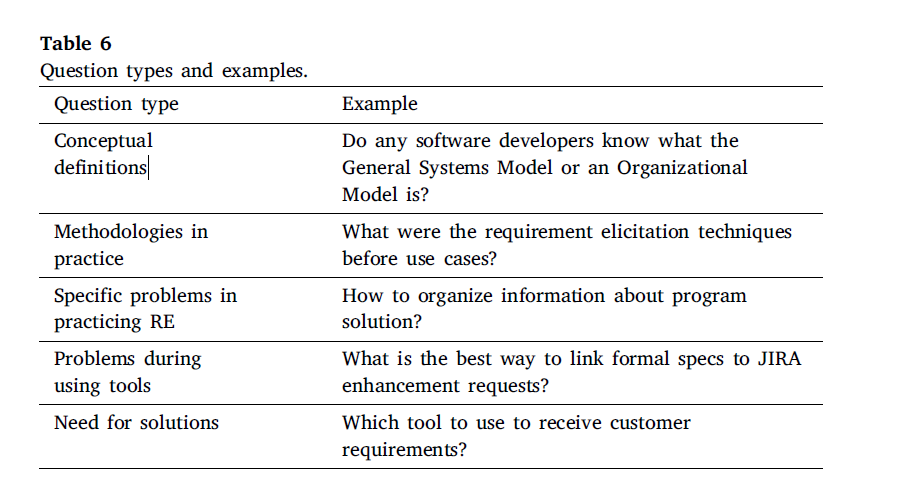
\includegraphics[width=0.5\textwidth]{Image/table-6.png}
                \end{figure}

            \subsubsection{تعداد پاسخ‌ها}

                ما به صورت سیستماتیک تعداد پاسخ‌های مربوط به ۳۷۵ سوال از Stack Overflow را ثبت کردیم. تنها ۲۱ از ۳۷۵ سوال بدون پاسخ مانده‌اند. همه این سوالات مجموعاً ۶۶۵ پاسخ دریافت کرده‌اند، با میانگین ۱.۸ پاسخ به ازای هر سوال.

            \subsubsection{وضعیت سوالات}

                از میان ۳۷۵ سوال، بیشتر سوالات (۳۵۴) پاسخ دریافت کرده‌اند، با ۱۹۶ سوال که پاسخ‌ها را پذیرفته‌اند. ۱۷۹ سوال باقی‌مانده که پذیرفته نشده‌اند، ممکن است نشان‌دهنده این باشد که سوال‌پرسندگان از پاسخ‌های موجود ناراضی هستند یا منتظر راه‌حل‌های رضایت‌بخش‌تر هستند.

        \subsection{حوزه مشکل}

            در این بخش، فعالیت‌ها و وظایف RE که در هر نوع سوال ذکر شده‌اند را معرفی می‌کنیم تا توجه جامعه Stack Overflow به RE را نشان دهیم.

            تعاریف مفهومی: سوالات مربوط به تعاریف مفهومی به تعریف یک یا چند مفهوم خاص RE می‌پردازند. به طور خاص، ۲۷ سوال در مجموع ۱۶ مفهوم RE را ۴۱ بار ذکر کرده‌اند. یازده مفهوم تنها یک بار ذکر شده‌اند که ۲۶.۸۳٪ از کل ذکرها (۱۱/۴۱) را تشکیل می‌دهند. مفاهیم که بیشترین فراوانی را دارند، نیازمندی‌های عملکردی (FR)، موارد استفاده، و نیازمندی‌ها هستند. FR در یازده سوال، موارد استفاده و نیازمندی‌ها هر کدام در شش سوال جداگانه ظاهر شدند. قابل توجه است که شش سوال به طور مستقیم درباره تعریف نیازمندی‌های غیرعملکردی پرسیده‌اند.

            بر اساس یافته‌های ما، سوالات تعاریف مفهومی را به دو دسته تقسیم می‌کنیم: سوالاتی که به تعریف یک مفهوم خاص می‌پردازند و سوالاتی که تفاوت بین دو یا چند مفهوم را مشخص می‌کنند. از این میان، سوالاتی که تفاوت بین مفاهیم را مشخص می‌کنند، بیشتر هستند و شامل ۲۲ سوال (۸۱.۵٪ از کل سوالات تعاریف مفهومی) می‌شوند. مفاهیمی که بیشترین تمایز را دارند، FR و NFR هستند که پنج سوال تفاوت این دو مفهوم را مشخص می‌کنند. علاوه بر این، سه سوال تفاوت بین FR و موارد استفاده را مشخص می‌کنند. پنج سوال دیگر به تعریف چهار مفهوم مختلف می‌پردازند: نیازمندی‌های منطقی، انواع نیازمندی‌ها، موارد استفاده غیرعملکردی، و نیازمندی‌های عملکردی غیر تعاملی.

            روش‌شناسی‌ها در عمل: ۸۳ سوال در مورد روش‌شناسی‌های RE مربوط به ۲۴ فعالیت RE پرسیده شده است. از این میان، نزدیک به یک سوم (۳۰/۸۳، ۳۶.۱٪) مربوط به تحلیل بودند، پس از آن تعیین مشخصات (۲۴/۸۳، ۲۸.۹٪) و مدیریت (۲۲/۸۳، ۲۶.۵٪) قرار دارند. تعداد سوالات مربوط به فعالیت‌های استخراج و اعتبارسنجی به ترتیب ۵ و ۲ سوال بود.

            برای وظایف RE، ابتدا چند وظیفه اصلی را معرفی می‌کنیم. متداول‌ترین وظیفه نوشتن نیازمندی‌ها در فعالیت تعیین مشخصات است که در مجموع ۱۴ سوال دارد. بعد از آن ایجاد مشخصات و تحلیل نیازمندی‌های مبتنی بر رفتار هر کدام با ۸ سوال قرار دارند. سپس مدل‌سازی نیازمندی‌ها با ۷ سوال قرار دارد.

            مشکلات خاص در اجرای RE: ۱۳۷ فعالیت RE در سوالات مربوط به مشکلات خاص در اجرای RE وجود دارند. فعالیت RE با بیشترین تعداد سوال، فعالیت تحلیل با ۸۴ سوال (۷۲/۱۲۴، ۶۱.۳٪) است. دومین فعالیت پر تکرار فعالیت تعیین مشخصات با ۳۳ سوال است.

            برای وظایف RE، مدل‌سازی نیازمندی‌ها بیشترین تعداد سوال با ۳۲ سوال را دارد. سپس طبقه‌بندی نیازمندی‌ها با ۱۴ سوال و نوشتن نیازمندی‌ها با ۱۲ سوال قرار دارند، در حالی که سایر وظایف در تحلیل و دیگر فعالیت‌های RE هر کدام کمتر از ۱۰ سوال دارند.

            مشکلات در استفاده از ابزارها: فعالیت RE متداول‌ترین در مدیریت است که در ۷۸ سوال ذکر شده است. پس از آن، تعیین مشخصات، تحلیل و اعتبارسنجی به ترتیب در ۶، ۶ و ۲ سوال ذکر شده‌اند.

            به دلیل تفاوت بین تعداد سوالات در مدیریت و تعداد سوالات در چهار فعالیت باقی‌مانده، ما فقط وظایف خاص مرتبط با فعالیت مدیریت را شمارش می‌کنیم. متداول‌ترین وظیفه مدیریت، CRUD نیازمندی‌ها است که ۲۱ سوال مرتبط با آن است، که تقریباً یک سوم از تمام سوالات مرتبط با فعالیت‌های مدیریت را تشکیل می‌دهد. دومین وظیفه، پیگیری نیازمندی‌ها با ۱۷ سوال است.

            نیاز به راه‌حل‌ها: روش‌هایی که کاربران درخواست می‌کنند را می‌توان به ابزارهای RE و تکنیک‌های ML دسته‌بندی کرد که در اینجا به طور کلی به عنوان راه‌حل‌ها نامیده می‌شوند. برای فعالیت‌های RE، متداول‌ترین مورد تحلیل است که در ۱۶ سوال ذکر شده است. بعد از آن، مدیریت با ۱۲ سوال قرار دارد.

            سپس، چهار وظیفه اصلی RE را معرفی می‌کنیم. وظیفه‌ای که بیشترین تعداد سوالات در مورد ابزارهای نیازمندی‌ها را دارد، پیگیری نیازمندی‌ها است که ۶ سوال در مورد آن است. پس از آن ایجاد مشخصات با ۳ سوال قرار دارد. دو مورد آخر پیگیری نیازمندی‌ها و مدیریت مستندات نیازمندی‌ها هستند که هر کدام در ۲ سوال ذکر شده‌اند.

            \begin{figure}
                \centering
                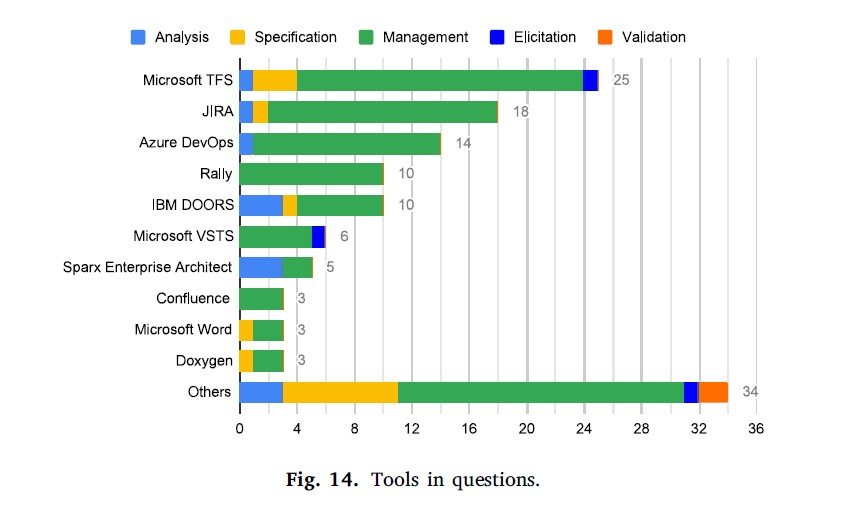
\includegraphics[width=0.5\textwidth]{Image/fig-14.jpg}
            \end{figure}

    \subsection{حوزه راه‌حل}

        در این زیربخش، ابزارها و روش‌های یادگیری ماشین مورد استفاده برای حل مشکلات مهندسی نیازمندی‌ها در جامعه Stack Overflow معرفی می‌شود.

        \subsubsection{ابزارها}
        
            ابزارها در سوالات: ما تمام ابزارهای مهندسی نیازمندی‌ها که در 375 سوال ذکر شده‌اند را شمارش کرده‌ایم. مجموعاً، 80 سوال (22.7\% از کل، 85/375) به 40 ابزار مختلف 130 بار اشاره کرده‌اند. شکل ۱۴ آمار را نشان می‌دهد و ابزارهایی که فقط یک بار ذکر شده‌اند با عنوان "دیگر" مشخص شده‌اند. پرکاربردترین ابزاری که در سوالات ذکر شده است Microsoft TFS است که در 25 سوال اشاره شده است و بیشترین استفاده آن در فعالیت‌های مدیریت نیازمندی‌ها اتفاق افتاده است. به دنبال آن، Atlassian Jira و Azure DevOps به ترتیب در 18 و 14 سوال ذکر شده‌اند که هر دو برای فعالیت مدیریت نیازمندی‌ها استفاده می‌شوند. از شکل مشخص است که بیشترین ابزارهای مورد اشاره در سوالات برای فعالیت‌های مدیریت نیازمندی‌ها استفاده می‌شوند.

            ابزارها در پاسخ‌ها: ما تمام ابزارهای مورد ذکر در 665 پاسخ را شمارش کرده‌ایم. مجموعاً، 148 پاسخ (23.49\% از کل، 148/665) به 98 ابزار مختلف 206 بار اشاره کرده‌اند، به متوسط 1.4 ابزار برای هر پاسخ (206/148). برای هر ابزار، تعداد پاسخ‌هایی که آن را ذکر کرده‌اند را شمرده‌ایم. شکل ۱۵ نتایج را نشان می‌دهد و ابزارهایی که فقط یک بار ذکر شده‌اند با عنوان "دیگر" مشخص شده‌اند. پرکاربردترین ابزاری که در پاسخ‌ها ذکر شده است Atlassian Jira است که در 25 پاسخ اشاره شده است و به دنبال آن Microsoft TFS و Rally با 18 و 12 پاسخ به ترتیب ذکر شده‌اند. بیشتر این ابزارهای برتر که در پاسخ‌ها ذکر شده‌اند برای فعالیت مدیریت نیازمندی‌ها مورد استفاده قرار می‌گیرند.

            \begin{figure}
                \centering
                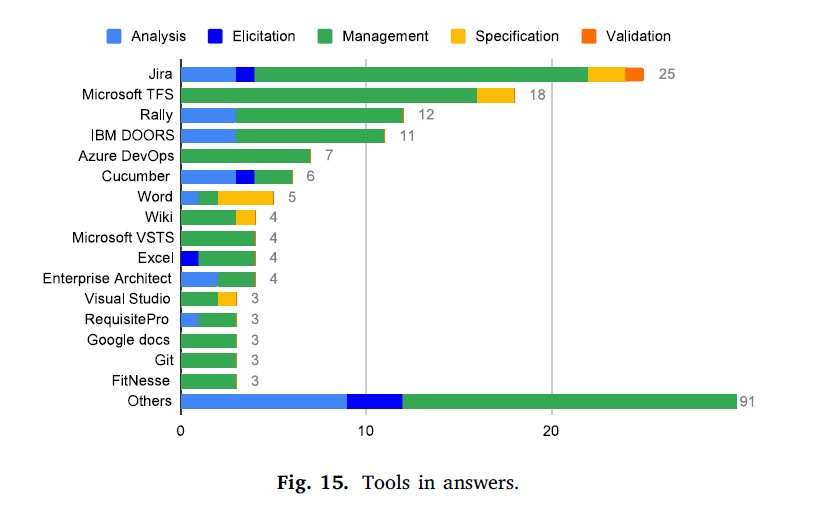
\includegraphics[width=0.5\textwidth]{Image/fig-15.jpg}
            \end{figure}

            \subsubsection{یادگیری ماشین}
            
                انواع وظایف ML: ما انواع وظایفی که توسط ML در سوالات انتخاب شده و پاسخ‌های متناظر با آنها ذکر شده را ثبت کرده‌ایم که شامل 35 سوال و 28 پاسخ می‌شود. در میان تمام وظایف ML مورد ذکر، بیشترین تمرکز بر روی دسته‌بندی است، که به ترتیب توسط خوشه‌بندی و مدل‌سازی موضوع دنبال می‌شود.

                تکنیک‌های ML: در میان 35 سوال و پاسخ متناظر که انتخاب کرده‌ایم، 14 تکنیک ML مختلف به طور کلی 36 بار ذکر شده‌اند. پرکاربردترین تکنیک‌های ML که به ترتیب 5 بار ذکر شده‌اند شامل LDA، POS tagging و TF–IDF هستند، که به دنبال آن شبکه‌های عصبی و GSDMM (4 بار هر کدام) و سپس k-NN (3 بار) می‌آیند. مشاهده می‌شود که عمده از تکنیک‌های ML استفاده شده توسط عمل‌گرایان مربوط به پردازش متن است.

                ابزارهای ML: در میان 35 سوال و پاسخ متناظر که انتخاب کرده‌ایم، 13 ابزار ML مختلف به طور کلی 38 بار ذکر شده‌اند. پرکاربردترین ابزارهای ML که ذکر شده‌اند scikit-learn (8 بار)، gensim (7 بار) و سپس textblob و tm (4 بار هر کدام) هستند.

        \subsection{داده}

            در این زیربخش، وضعیت داده‌های حوزه مهندسی نیازمندی‌ها که توسط جامعه Stack Overflow پردازش شده است، معرفی می‌شود. باید توجه داشت که به دلیل اشاره کمتر به داده‌ها در سوالات نسبت به بخش سفید، ما فقط انواع داده‌ها را اینجا استخراج کردیم. از تحلیل ما، تمام داده‌های مورد استفاده در این سوالات شامل آثار نیازمندی و صداهای کاربری است. به طور خاص، بیشترین داده‌های مورد اشاره داستان کاربری است که حدود 37.6\% (141/375) از کل داده‌ها را تشکیل می‌دهد. داده‌های دیگر اغلب شامل نیازمندی‌ها، توییت‌ها، مورد استفاده و اسناد نیازمندی‌ها هستند.

        \subsection{وضعیت عملیات ML4RE در Stack Overflow}

            خلاصه، تعداد کلیه سوالات مرتبط با نیازمندی‌های انتظاری کاهش یافته است. در حالی که تعداد قابل توجهی از سوالات پاسخ داده شده‌اند، تنها بخش محدودی از آنها پذیرفته شده‌اند. تمرکز اصل  این سوالات بر انالیز و فعالیت‌های مدیریت می‌چرخد، با وظایف خاصی مانند مدل‌سازی نیازمندی‌ها، نوشتن نیازمندی‌ها و پیگیری نیازمندی‌ها. ابزارهای مورد اشاره در پاسخ‌ها و سوالات شامل Microsoft TFS، Jira، IBM Rational DOORS، Rally و Azure DevOps هستند، در حالی که تکنیک‌های ML شامل LDA، POS، TF–IDF و شبکه‌های عصبی هستند. نوع اکثریت داده‌های مورد اشاره در سوالات آثار نیازمندی است و داستان‌های کاربری بیشترین تکرار را دارند.

            \begin{figure}
                \centering
                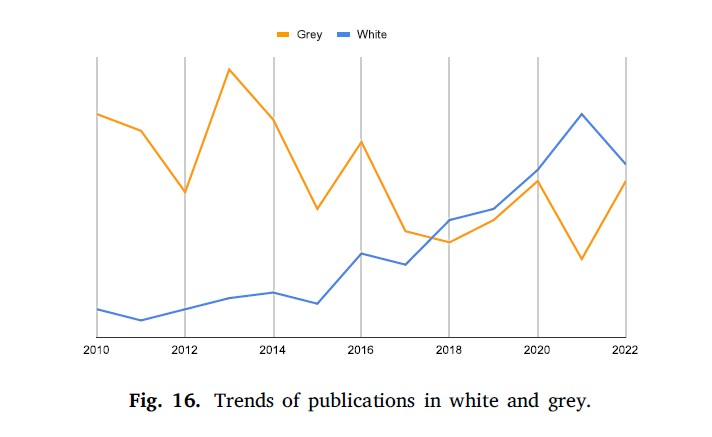
\includegraphics[width=0.5\textwidth]{Image/fig-16.jpg}
            \end{figure}
    
    % MARK: Joint part results (RQ3)

    \section{نتایج بخش مشترک (RQ3)}
    
        با توجه به طراحی در بخش 3.4.3، ما نتایج مقایسه‌ای از بخش‌های سفید و خاکستری را برای پاسخ به RQ3 ارائه می‌دهیم.

        \subsection{اطلاعات پایه}
        
            در این زیربخش، ما روندهای مختلف بخش‌های سفید و خاکستری در حوزه ML4RE را در شکل ۱۶ مقایسه می‌کنیم.

            در کل، یک روند صعودی در تعداد مقالات و یک روند نزولی در تعداد سوالات وجود دارد. به طور خاص، بین سال‌های 2010 تا 2013، هر دو بخش سفید و خاکستری روند صعودی را نشان دادند. با این حال، از سال 2014 تا 2017، بخش خاکستری نشان‌دهنده یک روند نزولی بود در حالی که بخش سفید نشان دهنده یک روند صعودی بود. سپس، در سال‌های بعدی، بخش سفید ادامه داد به آرامی افزایش یابد در حالی که بخش خاکستری به طور نسبی ثابت ماند.

        \subsection{حوزه مسئله}

            برای تجزیه و تحلیل تمرکز تحقیقات دانشگاهی و کاربردهای واقعی در حوزه مهندسی نیازمندی‌ها، ما فعالیت‌های RE و وظایف RE در بخش‌های سفید و خاکستری را مقایسه می‌کنیم.

            \subsubsection{فعالیت‌های RE}

                ما درصد هر فعالیت RE در بخش‌های سفید و خاکستری را مقایسه می‌کنیم. تحلیل RE نسبت به همه بخش‌ها بیشترین درصد را به خود اختصاص داده است، حدود 40\%. در مقابل، درصد سایر فعالیت‌های RE تفاوت واضحی را نشان می‌دهد. به طور خاص، در بخش سفید، هیچ کدام از مقالات به مشخصات RE پرداخت نکردند. با این حال، 19\% از سوالات در بخش خاکستری مربوط به این فعالیت بودند. مدیریت RE دومین فعالیت متداولی است که در بخش خاکستری مورد پوشش قرار گرفته است، با 32\% از سوالات. با این حال، فقط 11\% از مقالات در بخش سفید به این موضوع پرداخته‌اند. برای استخراج RE و اعتبارسنجی RE، بخش سفید به ترتیب حدود 26\% و 17\% را تشکیل می‌دهد. با این حال، تنها حدود 5\% و 3\% از سوالات در بخش خاکستری به این دو فعالیت ارتباط داشتند.

                برای درک دقیق‌تر از تمرکز بر فعالیت‌های RE بین بخش‌های سفید و خاکستری، ما روندهای فعالیت‌های RE را در این دو بخش مقایسه می‌کنیم، که در شکل ۱۷ نشان داده شده است. تحلیل به عنوان بیشترین فعالیت تاکید شده در هر دو بخش مشخص است. الگوگیری و اعتبارسنجی، در حالی که نمایش یک روند کلی افزایشی در بخش سفید از 2010 تا 2022 دارند، در بخش خاکستری توجه قابل توجهی نداشته‌اند. به علاوه، مدیریت به طور چشمگیری در بخش خاکستری برجسته است که یک روند پایدار در طول سال‌ها نشان می‌دهد، در حالی که بخش سفید علاقه قابل توجهی به این فعالیت نداشته است. علاوه بر این، مشخصات نشان دهنده یک روند نزولی در بخش خاکستری است که در بخش سفید توجه کمتری را به خود جلب کرده است.

                \subsubsection{وظایف RE}

                    هشت وظیفه RE تلاقی شده بین بخش‌های سفید و خاکستری وجود دارد: مدل‌سازی نیازمندی‌ها، پیگیری نیازمندی‌ها، دسته‌بندی نیازمندی‌ها، استخراج نیازمندی‌ها، ارزیابی کیفیت نیازمندی‌ها، اولویت‌بندی نیازمندی‌ها، انتخاب تکنیک استخراج نیازمندی‌ها و بازیافت و تولید نیازمندی‌ها. ما این وظایف را بر اساس تعداد تکرار آنها در بخش‌های سفید و خاکستری رتبه‌بندی می‌کنیم، که به ما امکان می‌دهد توجه نسبی آنها را در هر دو منطقه مشخص کنیم. وظایفی که مورد توجه هر دو بخش قرار می‌گیرند شامل مدل‌سازی نیازمندی‌ها و دسته‌بندی نیازمندی‌ها هستند. با این حال، ارزیابی کیفیت نیازمندی‌ها فقط در بخش سفید مورد توجه قرار می‌گیرد، در حالی که پیگیری نیازمندی‌ها فقط در بخش خاکستری تمرکز دارد.

            \subsection{حوزه راه‌حل}

                ما شباهت‌ها و تفاوت‌های روش‌های استفاده شده توسط تحقیقات دانشگاهی و کاربر

                دهای واقعی در Stack Overflow برای حل مسائل در RE را در این زیربخش مورد تجزیه و تحلیل قرار می‌دهیم.

                در بخش سفید، تکنیک‌های ML مورد استفاده فراوان عبارتند از SVM، CNN، درخت تصمیم، Bert، جنگل تصادفی و BiLSTM. سپس، ما یک جمع‌بندی جامع از ابزارهایی که در سوالات و پاسخ‌ها ظاهر شده‌اند را تهیه کرده‌ایم، که شناسایی ابزارهای بیشترین تکرار را همچون Microsoft TFS، Jira، IBM Rational DOORS، Rally و Azure DevOps می‌سازد. علاوه بر این، برخی از تکنیک‌های ML در بخش‌هایی از سوالات و پاسخ‌ها ذکر شده‌اند، به ویژه شامل LDA، POS، TF–IDF و شبکه‌های عصبی هستند. بنابراین، مشاهده می‌شود که تمرکز بخش سفید بر روی روش‌های سنتی طبقه‌بندی و رگرسیون و همچنین مدل‌های یادگیری عمیق است. از سوی دیگر، تمرکز بخش خاکستری شامل ابزارهای نرم‌افزار معمول و برخی از تکنیک‌های ML مرتبط با تحلیل متن و پردازش زبان طبیعی است.

        \subsection{داده}

            ما نوع داده عمومی و داده خاص استخراج‌شده از بخش‌های سفید و خاکستری را مقایسه می‌کنیم تا توجه آن‌ها به داده‌ها را تجزیه و تحلیل کنیم.

            متداول‌ترین نوع داده عمومی در هر دو بخش سفید و خاکستری آثار نیازمندی‌ها است. ما مصرف 6 نوع داده خاص بالاترین را در داخل آرتیفکت‌های نیازمندی در بین دو بخش مقایسه می‌کنیم، که در شکل ۱۸ نشان داده شده است. در بخش سفید، بیشترین استفاده از نیازمندی‌ها و اسناد نیازمندی‌ها است و این دو نوع همچنین به طور متداول در بخش خاکستری استفاده می‌شوند. در میان سایر انواع داده در بخش خاکستری، داستان کاربر و مورد استفاده به توجه قابل توجهی رسیده‌اند، به ویژه داستان کاربر. با این حال، در بخش سفید، توجه کمتری به این دو نوع داده وجود دارد.
            

        \subsection{شباهت‌ها و تفاوت‌های بین تحقیقات دانشگاهی و کاربردهای Stack Overflow}

            خلاصه‌اش، در حالی که تعداد مقالات علمی افزایش یافته است، سوالات منتشر شده در جامعه Stack Overflow کاهش یافته است. هر دو بخش تاکید دارند بر تحلیل نیازمندی‌ها، مدل‌سازی نیازمندی‌ها و دسته‌بندی نیازمندی‌ها. با این حال، دانشگاه تأکید دارد بر استخراج و اعتبارسنجی نیازمندی‌ها با استفاده از تکنیک‌های ML مانند SVM، CNN، درخت تصمیم و BERT. بر عکس، جامعه Stack Overflow بیشتر تمرکز خود را بر مدیریت و مشخصات نیازمندی می‌گذارد، با استفاده از ابزارهایی مانند Microsoft TFS، Jira، IBM Rational DOORS، Rally و Azure DevOps، و همچنین تکنیک‌های ML مانند LDA، POS، TF–IDF و شبکه‌های عصبی. در مورد داده، در حالی که هر دو توجه دارند به نیازمندی‌ها و اسناد نیازمندی، جامعه Stack Overflow به طور خاص تأکید دارد بر داستان کاربر و مورد استفاده که در تحقیقات علمی کمتر مورد توجه قرار گرفته‌اند.

    % MARK: Discussion

    \section{بحث}

        در این بخش، ابتدا پدیده‌های جالبی که بر اساس نتایج پژوهش ما به دست آمده است را ارائه و تحلیل می‌کنیم. سپس با استفاده از این تحلیل‌ها، یک مجموعه پیشنهادات پژوهشی ارائه می‌دهیم.

        \begin{figure}
            \centering
            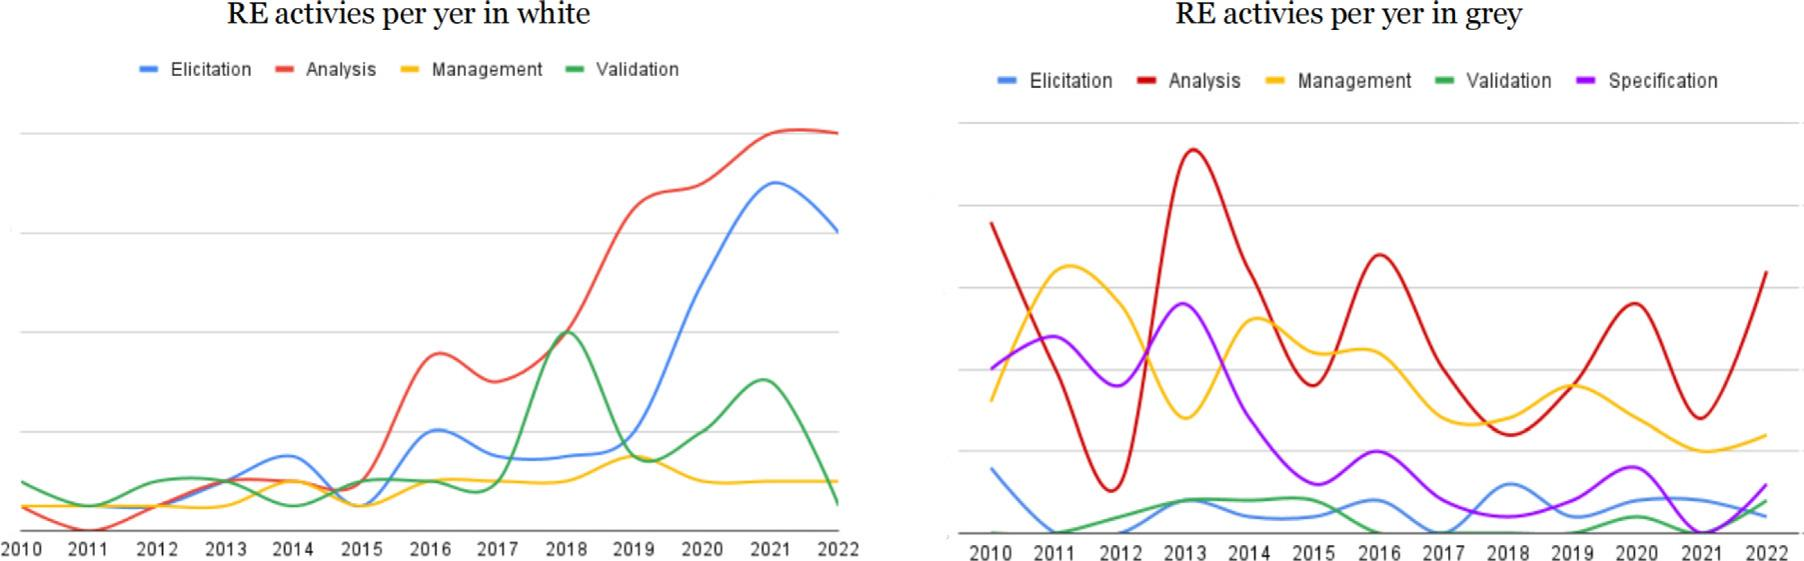
\includegraphics[width=0.5\textwidth]{Image/fig-17.jpg}
            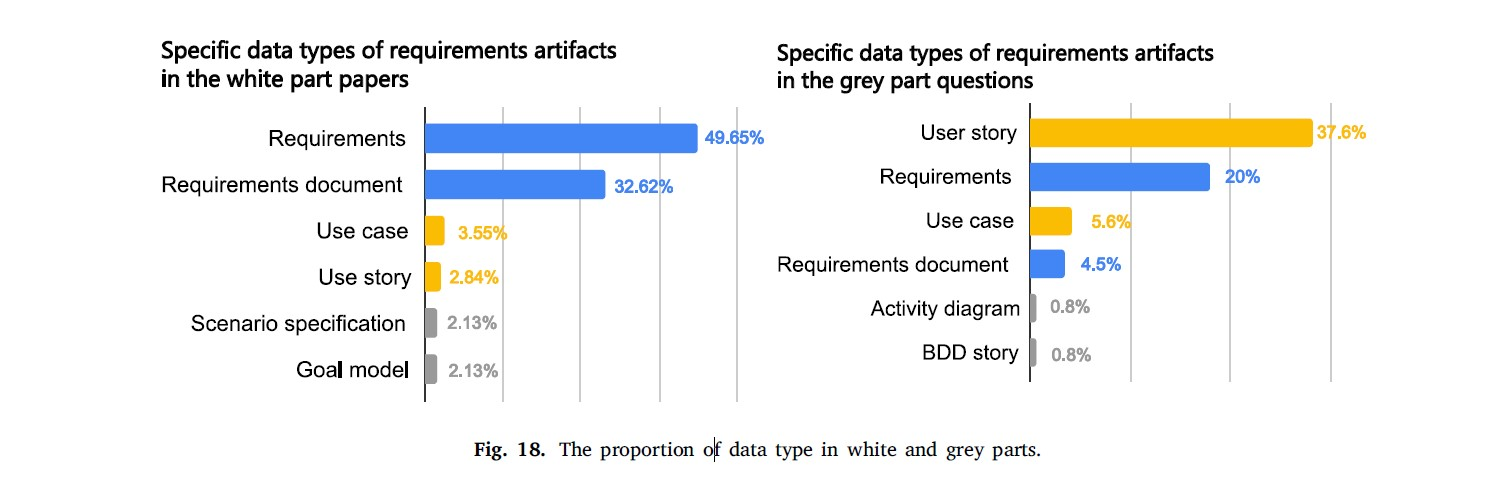
\includegraphics[width=0.5\textwidth]{Image/fig-18.jpg}
        \end{figure}

        \subsection{سوار شدن بر موج پیشرفت‌های فناورانه}

            هنگام تجزیه و تحلیل مقالات انتخاب شده، ما تمایلات و تغییرات مهمی که به پیشرفت تکنولوژی مرتبط هستند مشاهده کردیم. ابتدا، ما افزایش قابل توجهی در تعداد مقالات مرتبط با ML4RE مشاهده کردیم. این روند با توسعه سریع تکنیک‌های یادگیری ماشین همخوانی دارد و همچنین با روند رشد تعداد برنامه‌ها در 13 سال گذشته همبستگی دارد [40، 41]. با افزایش تعداد برنامه‌ها، تقاضا برای برجسته شدن در بازار رقابتی اهمیت زیادی پیدا می‌کند، که نیازمندی‌ها را حیاتی‌تر می‌سازد. هم‌زمان، این افزایش منجر به ایجاد حجم زیادی از داده‌های قابل تحلیل شده است، که فناوری ML به عنوان یک روش تحلیلی موثر، پژوهش در ML4RE را رهبری می‌کند.

            مقالات انتخاب شده همچنین در طول مسیر واضحی را با تکامل فناوری یادگیری ماشین دنبال کرده‌اند. ما نقشه راه را به عنوان در شکل ۱۹ نشان داده شده است خلاصه می‌کنیم. در فاز اولیه، از 2010 تا 2015، تمرکز اصلی به الگوریتم‌های سنتی یادگیری ماشین مانند SVM و روش‌های بیزین بود. سپس، حدود سال‌های 2016 تا 2017، تأکید پژوهش به سمت شبکه‌های عصبی بنیادی، مانند CNN، همراه با تکنیک‌های تعبیه کلمات مانند word2vec شیفت کرد. سپس، از سال 2017 تا 2019، افزایش قابل توجهی در استفاده از روش‌های یادگیری عمیق، به ویژه پذیرش LSTM، مشاهده شد. اخیراً، در بازه زمانی 2020 تا 2022، توجه به آرامی به سمت مدل‌های تولیدی و پیش‌آموزش‌داده‌شده مانند BERT و GPT معطوف شد. انتظار می‌رود که پژوهش‌های آینده در ML4RE به طور گسترده‌تری مدل‌های زبان بزرگ را بررسی کنند.

            علاوه بر این، هر چند داده عمومی به عنوان بزرگ‌ترین منبع داده باقی می‌ماند، اما رشد پژوهش‌هایی که از این داده‌ها استفاده می‌کنند در دو سال گذشته کاهش یافته است. به طور مقابل، افزایش قابل توجهی در مطالعاتی که از داده‌های کراول شده استفاده می‌کنند، مشاهده شده است. یک دلیل احتمالی برای این می‌تواند به دوران داده‌های بزرگ و پیشرفت فناورانه بازگردانده شود. حضور همیشگی فناوری دیجیتال در زندگی روزمره، مقدار زیادی از داده‌ها را تولید می‌کند که به پژوهشگران این امکان را می‌دهد که برای منابع داده مفهومی و واقع‌گرایانه‌تر برای مطالعات خود استفاده کنند.

            این مشاهدات در پاسخ به پیشرفت‌های فناورانه در تحقیقات ML4RE است و برای پژوهش‌های آینده، دستاوردها و راهنمایی‌های ارزشمندی فراهم می‌کند.

            \begin{figure}
                \centering
                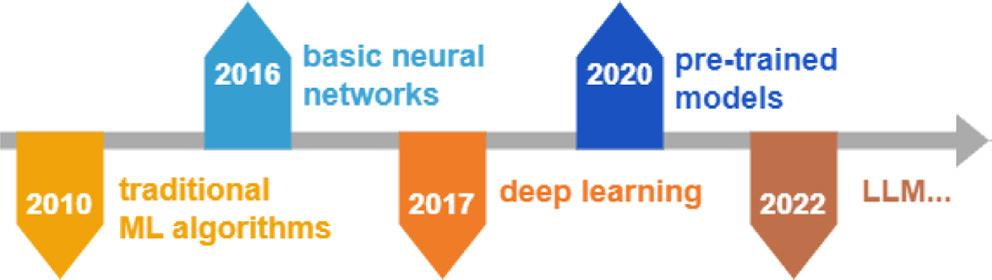
\includegraphics[width=0.5\textwidth]{Image/fig-19.jpg}
            \end{figure}

        \subsection{تضاد اولویت‌ها بین تحقیقات دانشگاهی و عملیات در Stack Overflow}

            در تحلیل مقایسه‌ای ما از تحقیقات دانشگاهی و عملیات در Stack Overflow در مورد مسائل در حوزه RE، یک اختلاف مشخص ظاهر می‌شود. بر اساس یافته‌ها، پژوهشگران تمایل دارند به استفاده از تکنیک‌های پیشرفته یادگیری ماشین و یادگیری عمیق (DL). به عنوان مقابل، مشاهده شده است که از نرم‌افزارهای موجود و تکنیک‌های پردازش زبان طبیعی (NLP) در عمل استفاده می‌شود.

            دلیل اصلی این اختلاف ممکن است در تأکید دانشگاهی بر نوآوری و پیچیدگی فناوری‌ها باشد، در حالی که صنعت بیشتر بر اهمیت عملیاتی و کارایی هزینه‌ای تأکید می‌کند.

            تکنیک‌های ML و DL که در بخش سفید استفاده می‌شوند، معمولاً شامل پیچیدگی و هزینه بالا هستند و نیاز به دانش تخصصی و حرفه‌ای برای توسعه و اجرا دارن

            د. علاوه بر این، این تکنیک‌ها معمولاً نیازمند مجموعه داده آموزشی قابل توجه و منابع محاسباتی هستند. در مقابل، ابزارهای نرم‌افزاری و تکنیک‌های NLP که در بخش خاکستری استفاده می‌شوند، معمولاً آسان‌تر برای پیاده‌سازی و کاربرد هستند، زیرا که از پیش در صنعت پذیرفته شده‌اند و دارای منحنی یادگیری و هزینه کمتری هستند.

            علاوه بر این، تنها بخشی از سوالات و پاسخ‌ها در بخش خاکستری به تکنیک‌های ML اشاره دارند. این ممکن است به دلیل برخی سوالات مربوط به تعریف مفاهیم، روش‌ها و ابزارهای RE باشد. بنابراین، تمرکز تنها بر دانش حوزه RE برای پاسخ به این سوالات کافی است. به علاوه، برخی از سوالات ممکن است شرایط خاصی را ارائه دهند، که پاسخ‌های آن‌ها بر اساس روش‌های خاصی طراحی شده برای آن شرایط باشد و نیازی به تکنیک‌های ML نداشته باشد.

        \subsection{عدم ارتباط بین تحقیقات دانشگاهی و عملیات صنعتی}

            در مقایسه تمرکز بر فعالیت‌های RE و داده بین بخش‌های سفید و خاکستری، اختلافاتی را که به عدم ارتباط بین دانشگاه و صنعت اشاره دارد، شناسایی کردیم.

            از شکل ۱۷، اختلاف در توجه در فعالیت‌های RE آشکار می‌شود. بخش خاکستری به طور مداوم برخی از سوالات مرتبط با مدیریت RE را مطرح می‌کند، در حالی که تحقیقات دانشگاهی در بخش سفید افزایش قابل توجهی در این حوزه نشان نمی‌دهد. این تفاوت ممکن است ناشی از کمبود ارتباط بین دانشگاه و صنعت باشد که منجر به عدم درک در دانشگاه درباره نیازها و جهت‌گیری‌های خاص در مدیریت RE شود.
            
            علاوه بر این، در شکل ۱۸، بخش خاکستری به توجه قابل توجهی به داستان کاربر و مورد استفاده اختصاص داده است، بخش‌هایی که در تحقیقات دانشگاهی کمتر توجه می‌شود. این عدم تأکید بر این جوانب در تحقیقات دانشگاهی نیز به ارتباط ممکن است که با حساسیت این داده‌ها در مورد حریم خصوصی شرکت‌ها مرتبط باشد که باعث می‌شود حمایت و داده کافی برای تحقیقات دانشگاهی مشکل باشد.

            کلیتاً در حالی که دانشگاه سعی در بررسی روش‌های نوین دارد، این رویکردها ممکن است همیشه با مشکلات عملی و نیازهای مستقیم صنعت همخوانی نداشته باشد. این اختلافات نیاز به هم‌آمیزی نزدیک‌تر بین جهت‌گیری‌های تحقیقی و نیازهای واقعی دنیای واقعی را نشان می‌دهد.

        \subsection{پیشنهادات}

        در این زیربخش، ما قصد داریم بر اساس یافته‌ها و بحث‌های خود چندین پیشنهاد برای پژوهشگران در زمینه ML4RE ارائه دهیم.

        \subsubsection{ساخت دستیاران هوشمند پاسخگوی سوال}

            با تحقیقات انجام شده در بخش خاکستری، مشخص شد که سوالات مربوط به مشکلات خاص در انجام RE و تعریف مفهوم، به ترتیب به نسبت 36.2\% و 8.2\%، اشغال کننده اولویت هستند. این نشان می‌دهد که برخی از سوالات می‌توانند با بهره‌گیری از دانش تخصصی در زمینه RE حل شوند. با توجه به پیشرفت‌های فناورانه فعلی، توسعه دستیاران هوشمند پاسخگوی سوال بر اساس مدل‌های زبان بزرگ (LLM) یک جهت تحقیقاتی پر امید است.

            LLM نمایانگر یک دسته از ابزارهای قدرتمند NLP هستند که از آموزش از پیش گسترده و تکنیک‌های یادگیری عمیق بهره می‌برند. این مدل‌ها توانایی درک عمیق، استدلال و تولید متن طبیعی را دارند. این قابلیت باعث می‌شود که LLM بتواند دانش را از داده‌های متنی گسترده استخراج کرده، زمینه را درک کند و بنابراین قادر به استدلال منطقی برای تولید پاسخ‌های دقیق باشد. بنابراین، ساخت دستیار پاسخگوی سوال با استفاده از LLM چندین مزیت متمایز ارائه می‌دهد: (۱) مخزن جامعی از دانش مخصوص حوزه که از آموزش گسترده LLM ناشی می‌شود؛ (۲

            ) توانایی درک و استدلال برتر که اجازه رفع مشکلات پیچیده RE را می‌دهد؛ (۳) پاسخگویی به صورت زمان واقعی و واکنش‌پذیری دقیق در ارائه پاسخ‌های مؤثر و دقیق به سوالات.

            با توجه به این مزایا، توصیه می‌شود که مجموعه‌داده‌ها را از دامنه RE سازماندهی کرده و سپس LLM را برای توسعه یک دستیار پاسخگوی سوال هوشمند بهبود دهیم. چنین دستیاری می‌تواند به طور مؤثری مفاهیم پیچیده‌ای را تشخیص دهد و حلول‌های مناسبی برای سوالات خاص RE ارائه دهد.


    % MARK: Threats to validity

    \section{تهدیدهای اعتبار}

        در این بخش، تهدیدهایی که ممکن است بر اعتبار کار ما تأثیر بگذارند، تجزیه و تحلیل می‌شود. در اینجا ما از یک روش دسته‌بندی براساس تحقیقات موردی در مهندسی نرم‌افزار توسط رونسون و هاست [۴۲] استفاده می‌کنیم که تمرکز آن بر روی مطالعات موردی در مهندسی نرم‌افزار است.

        \subsection{اعتبار ساختاری}

            اعتبار ساختاری نشان دهنده‌ی میزانی است که پروتکل تحقیق به اهداف و سوالات تحقیق می‌پردازد. نمایانگری مطالعات انتخاب شده مهمترین تهدید برای مطالعه ما است. برای بررسی ادبیات خاکستری، ما Stack Overflow را به عنوان منبع اطلاعات انتخاب کردیم. با این حال، در جستجوی با استفاده از ترکیبی از کلمات کلیدی RE و ML، نتایج به طور قابل توجهی محدود بودند. ما متوجه شدیم که سوالات بازیابی شده با استفاده از کلمات کلیدی RE به طور اصلی بر روی سناریوهای خاص متمرکز هستند و بنابراین پاسخ‌های مربوطه به این سناریوها عموماً به آنها تنظیم شده‌اند. با این حال، ما اعتقاد داریم که این سوالات همچنان به تجزیه و تحلیل چالش‌های RE در جهان واقعی کمک می‌کنند. بنابراین، ما تصمیم به انتخاب دو رویکرد برای جستجوی بخش خاکستری گرفتیم: یک‌سو، جستجوی سوالات مستقیماً مرتبط با RE و از سوی دیگر، ترکیب کلمات کلیدی ML با کلماتی که ارتباطی با RE دارند. ما متوجه هستیم که این روش جستجو ممکن است تمامی سوالات مرتبط با ML4RE را پوشش ندهد، اما ما تمام تلاش خود را برای تعادل بار کاری و کیفیت محتوا انجام داده‌ایم. ما منتظر جمع‌آوری منابع خاکستری جامع‌تر در تحقیقات آینده هستیم تا بررسی ادبیات ما را بیشتر غنی‌تر کنیم.
        
        \subsection{اعتبار داخلی}

            اعتبار داخلی نیازمند آن است که پژوهشگران به عواملی که بر تحقیق تأثیر می‌گذارند، به طور کامل توجه کنند. اگر یک عاملی وجود داشته باشد که بر کیفیت مطالعه تأثیر می‌گذارد و ما از آن اطلاع نداشته باشیم، تهدیدی برای اعتبار داخلی خواهد بود. طراحی بررسی ادبیات ما از راهنمایی‌های مقالات علمی استاندارد پیروی می‌کند که تا حدی از تهدیدات به اعتبار داخلی کاسته می‌شود. با این حال، تهدیدات احتمالی به اعتبار داخلی هنوز وجود دارد، به خصوص در خصوص دقت تگ‌گذاری دستی. در طول این فرآیند، نیاز به شمارش و استخراج حجم زیادی از داده‌ها وجود دارد. این وظایف می‌تواند خسته‌کننده باشد و ممکن است منجر به عدم دقت یا خطا در ثبت داده‌ها شود. برای کاهش این مشکل، ما یک صفحه‌کارگزاری مشترک ایجاد کرده، قوانین برچسب‌گذاری را تعریف کرده و نیاز به ورود دستی را کمینه کرده‌ایم، از این طریق خطر خطاهای پژوهشگران را کاهش می‌دهیم. به علاوه، ما داده‌ها را برای اطمینان از دقت آنها دوباره بررسی کرده و در محاسبات آماری هرگاه امکان داشته باشد از فرمول‌های محاسباتی استفاده می‌کنیم. ما اعتقاد داریم که این به کاهش تهدیدات در فرآیند جمع‌آوری داده‌ها کمک می‌کند.

        \subsection{اعتبار خارجی}

            اعتبار خارجی نمایانگر توانایی عمومی‌سازی نتایج مطالعه است. یک مشکل پتانسیلی با اعتبار خارجی ممکن است مربوط به فریم زمانی محدود داده باشد. در تجزیه و تحلیل ما، از داده‌های 2010 تا 2022، شامل هم ادبیات سفید و هم خاکستری استفاده کردیم، اما تحقیقات منتشر شده قبل از 2010 را در نظر نگرفتیم. خوشبختانه، پیشرفت سریع یادگیری ماشین از سال ۲۰۱۰ به بعد به کاهش این نگرانی کمک کرده است. یک تهدید دیگر ممکن است مربوط به دامنه محدود ادبیات خاکستری باشد. مشارکت اصلی ما در ارائه یک دید یکپارچه درباره ادبیات خاکستری است. Stack Overflow یکی از منابع اطلاعاتی اطلاعاتی و مناسب‌ترین است که به بهترین شکل نیازهای ما در این مقاله را می‌تواند برطرف سازد. ما تلاش کردیم تا شامل یک مجموعه گسترده از سوالات RE شویم تا تأثیر Stack Overflow به عنوان منبع اصلی داده را کاهش دهیم. با این حال، لازم است تا بپذیریم که قابلیت عمومی‌سازی یافته‌های ما ممکن است تحت تأثیر محدودیت‌های Stack Overflow باشد. برای پاسخ به این مسأله، کارهای آتی می‌توانند به تدریج منابع داده‌ای اضافی را به کار بگیرند تا اعتبار خارجی مطالعه ما را بهبود بخشند.

        \subsection{اعتبار استنباطی}

            اعتبار استنباطی مربوط به قابل تکرار بودن مطالعه است. این به این معنی است که آیا دیگر پژوهشگرانی که پروتکل مقاله ما را دنبال می‌کنند و مطالعات مشابه‌ای را انجام می‌دهند، می‌توانند نتایج مشابهی را به دست آورند؟ یک تهدید ممکن مربوط به جنبه‌هایی می‌تواند که به انتخاب داده مربوط باشد. برای کاهش این تهدید، ما معیارهای اضافه و حذف مشخص را برای داده‌ها در بخش‌های سفید و خاکستری معرفی کرده‌ایم و آنها را به طور سختگیرانه اعمال کرده‌ایم. دو نویسنده فرآیند انتخاب داده‌ها را کامل کردند و یک مطالعه پیش‌نمونه را برای هماهنگی نظرات خود قبل از شروع انجام دادند. ما یک پژوهشگر سوم را برای حل اختلافات بین دو نویسنده معرفی کردیم. یک تهدید مشابه در فرآیند برچسب‌گذاری داده‌های پس از آن وجود دارد. قبل از آنکه ما فرآیند داده‌برداری را شروع کنیم، ما به طور واضح تعریف کرده‌ایم که چه داده‌هایی را نیاز داریم و چگونه آنها را استخراج کنیم تا این تهدید را کاهش دهیم. مانند انتخاب مقاله، دو نویسنده فرآیند را کامل کرده‌اند و فرآیند حل اختلافات مشابهی را که در انتخاب مقاله انجام دادیم، دنبال کرده‌اند. علاوه بر این، محققان برچسب‌گذاری استاندارد را برای برچسب‌گذاری ایجاد کرده‌اند و از معیارهای دقیق اضافه/حذف برای اتحاد تفاوت‌ها بین محققان مختلف استفاده کرده‌اند. به طور خاص، دو محقق به طور همزمان برچسب‌گذاری مقاله را انجام دادند و به طور دوره‌ای تگ‌های خود را به یکدیگر ادغام کردند، زیرا اصطلاحات مختلف استخراج شده از مقالات مختلف ممکن است به یک چیز اشاره کنند. علاوه بر این، اعتبار بخش نقشه‌برداری برای اطمینان از اینکه تفسیر داده‌ها به عنوان یک معیار اشیایی و مطابق با معنی اصلی داده‌های استخراج شده انجام شده است، حیاتی است. ما چندین بحث و تغییرات در ارائه داده‌ها انجام دادیم تا اطمینان حاصل کنیم که نمودارهای نهایی نمایانگر اراده اصلی داده‌های استخراج شده هستند.

    % MARK: Conclusion and future work

    \section{نتیجه‌گیری و کارهای آینده}

        در این مقاله، یک بررسی منظم از ادبیات ML4RE با یکپارچگی دیدگاه‌های اجرایی از Stack Overflow انجام دادیم. به سوی علمیه، ما به طور سیستماتیک از چهار پایگاه داده علمی (IEEE Xplore، ACM Digital Library، SpringerLink و Scopus) جستجو کردیم و مقالات علمی مرتبط با ML4RE از سال ۲۰۱۰ تا ۲۰۲۲ را انتخاب و انتخاب کردیم. ما ۲۰۷ مقاله منتشر شده در زمینه ML4RE دریافت کردیم. برای ادبیات خاکستری، ما به طور سیستماتیک از Stack Overflow جستجو کردیم و ۳۷۵ سوال توسط اجرایی‌ها در تمرینات RE از سال ۲۰۱۰ تا ۲۰۲۲ با پاسخ‌های این سوالات را دریافت کردیم. ما روندهای ادبیات، فعالیت‌های RE، وظایف RE، راه‌حل‌ها و داده‌ها را تجزیه و تحلیل می‌کنیم. با تجزیه و یکپارچه‌سازی اطلاعات استخراج شده، وضعیت فعلی ML4RE در تحقیقات علمی و اجرایی در Stack Overflow را ارائه می‌دهیم. در نهایت، ما نتایج این دو بخش را مقایسه می‌کنیم تا شباهت‌ها و تفاوت‌های آنها را تشخیص دهیم. بر اساس نتایج تحقیقات ما، ما برخی از پدیده‌های جالب در ML4RE را بحث می‌کنیم که شایسته توجه هستند و پیشنهاداتی برای تحقیق ارائه می‌دهیم.

        کارهای آینده ما می‌تواند ادامه دادن جریان‌های تحقیقاتی جدید در این زمینه را شامل شود. علاوه بر این، ممکن است ادبیات خاکستری بیشتری درگیر شود تا به طور کامل به صداهای اجرایی‌ها و صنعت گوش داده شود.


\end{document}